% !TeX spellcheck = de_DE
% English option for spellcheck: en_US
\documentclass[%
FTMstudentthesis%		baseclass
,optArial%				font setting (alternative fonts for debugging purposes: optHelvetica, optCharter)
,optBiber%				bibliography tool (alternative: optBibtex)
,optGerman%				[optional] deutsche Vorlage: optGerman, english version: optEnglish
%,optTikzExternalize%	[optional] compiles faster for large tikz images
%,optHideTodos%			[optional] disables the todonotespackage and hides any todos and missingfigures
%,optGroupedAbbreviation%	[optional] gruppieren der Abkürzungen nach Buchstaben	
,optCMYK%					printing text pages as black and white
]{FTMlatex}%
%
%
% FTM: Definitions for the supported programming languages (including the possbility to add further keywords which are being highlighted in the code snippets):
\lstdefinelanguage{FTMsql}{%
	language     = SQL,%
	morekeywords = {AUTOINCREMENT, REFERENCES, RENAME, CHANGE, MODIFY, TRUNCATE, TEXT}%
}
\lstdefinelanguage{FTMpython}{%
	language     = Python,%
	morekeywords = {}%
}
\lstdefinelanguage{FTMjava}{%
	language     = Java,%
	morekeywords = {}%
}
\lstdefinelanguage{FTMc}{%
	language     = C,%
	morekeywords = {}%
}
\lstdefinelanguage{FTMcpp}{%
	language     = C++,%
	morekeywords = {}%
}
%
% Set paths
\graphicspath{{figures/}}%
\addbibresource{source/bibliography/literature.bib}%
\addbibresource{source/bibliography/bibliographyTest.bib}%
\makenoidxglossaries%
\newacronym{px}{px}{Pixel}%
\newacronym{GPU}{GPU}{Graphics Processing Unit}% done
\newacronym{CPU}{CPU}{Central Processing Unit}% done
\newacronym{RAM}{RAM}{Random Access Memory}%
\newacronym{ROS2}{ROS2}{Robot Operating System}% done
\newacronym{TF}{TF}{Transform System}% done
\newacronym{BM}{BM}{Block Matching}% done
\newacronym{SGM}{SGM}{Semi-Global Matching}% done
\newacronym{VO}{VO}{Visual Odometry}% done
\newacronym{PnP}{PnP}{Perspective-n-Point}% done
\newacronym{ORB}{ORB}{Oriented FAST and Rotated BRIEF}% done
\newacronym{FAST}{FAST}{Features from Accelerated Segment Test}% done
\newacronym{BRIEF}{BRIEF}{Binary Robust Invariant Scalable Keypoints}% done
\newacronym{RANSAC}{RANSAC}{Random Sample Consensus}% done
\newacronym{KF}{KF}{Kalman Filter}% done
\newacronym{EKF}{EKF}{Extended Kalman Filter}% done
\newacronym{CUDA}{CUDA}{Compute Unified Device Architecture}% done
\newacronym{SLAM}{SLAM}{Simultaneous Localization and Mapping}% done
\newacronym{TTC}{TTC}{Time to collision}% done
\newacronym{TSN}{TSN}{Time Sensitive Networking}%ompute Unifie done
\newacronym{PTP}{PTP}{Precision Time Protocol}%ompute Unifie done
\newacronym{LiDAR}{LiDAR}{Light Detection and Ranging}% done
\newacronym{RADAR}{RADAR}{Radio Detection and Ranging}% done
\newacronym{CNN}{CNN}{Convolutional Neural Network}% done
\newacronym{RNN}{RNN}{Recurrent Neural Network}% done
\newacronym{IMU}{IMU}{Inertial Measurement Unit}% done
\newacronym{GNSS}{GNSS}{Global Navigation Satellite System}% done
\newacronym{DBSCAN}{DBSCAN}{Density-Based Spatial Clustering of Applications with Noise}% done% Definition of Acronyms
%
%
\begin{document}%
%% ========================
%% ------ Title Page ------
%% ========================
\FTMPreText%
% Info: separate multiple supervisors by \newline
%\FTMstudentthesisTitlePageFTMDesignDiplomarbeit{Hier steht der Titel der Arbeit, der auch zweizeilig sein kann}{Hier kommt der englische Titel hin, der dann wohl auch zweizeilig sein muss}{Dipl.-Ing. Max Mustermann, B.Sc. \vskip0pt Musterweg 20 \vskip0pt 80999 München}{\FTMnamesProfLienkamp}{\FTMnamesStaffPonn}{\FTMutilsDate{31}{08}{2021}}{./figures/ImagePDF}%
%\FTMstudentthesisTitlePageFTMDesignBachelorsThesis{Hier steht der Titel der Arbeit, der auch zweizeilig sein kann}{Hier kommt der englische Titel hin, der dann wohl auch zweizeilig sein muss}{Dipl.-Ing. Max Mustermann, B.Sc. \vskip0pt Musterweg 20 \vskip0pt 80999 München}{\FTMnamesProfLienkamp}{\FTMnamesStaffPonn}{\FTMutilsDate{31}{08}{2021}}{./figures/ImagePDF}%
%\FTMstudentthesisTitlePageFTMDesignSemesterThesis{Hier steht der Titel der Arbeit, der auch zweizeilig sein kann}{Hier kommt der englische Titel hin, der dann wohl auch zweizeilig sein muss}{Dipl.-Ing. Max Mustermann, B.Sc. \vskip0pt Musterweg 20 \vskip0pt 80999 München}{\FTMnamesProfLienkamp}{\FTMnamesStaffPonn}{\FTMutilsDate{31}{08}{2021}}{./figures/ImagePDF}%
\FTMstudentthesisTitlePageFTMDesignMastersThesis{Hier steht der Titel der Arbeit, der auch zweizeilig sein kann}{Hier kommt der englische Titel hin, der dann wohl auch zweizeilig sein muss}{Dipl.-Ing. Max Mustermann, B.Sc. \vskip0pt Musterweg 20 \vskip0pt 80999 München}{\FTMnamesProfLienkamp}{Max Musterbetreuer, M.Sc.}{\FTMutilsDate{01}{10}{2021}}{./figures/ImagePDF}%
%
%
%% ========================
%% --- Student's Thesis ---
%% ========================
\hypersetup{pageanchor=false}
\vspace*{0cm}%
\FTMlayoutPutAtNorthWest{2.5cm}{1.5cm}{\FTMlogoTercetChair{1.05cm}}%
\FTMlayoutPutAtNorthEast{2.4cm}{2cm}{\FTMlogoTUM{1cm}{TUMBlue}}%

{\fontsize{24}{24} \selectfont \FTMlangProjectDescription}
\vspace{1cm}

{\fontsize{16}{18} \selectfont Titel der Arbeit}
\vspace{0,5cm}

Hier steht ein zum Thema hinführender Text.

In einer konstruktiven (oder theoretischen) \textcolor{red}{Bachelor/-Semester/-Masterarbeit} sollen (...)

Folgende Punkte sind durch \textcolor{red}{Herrn/Frau Martin Musterstudent} zu bearbeiten:

\begin{itemize}
	\item Punkt 1
	\item Punkt 2
\end{itemize}

Die Ausarbeitung soll die einzelnen Arbeitsschritte in übersichtlicher Form dokumentieren. Der Kandidat/Die Kandidatin verpflichtet sich, die \textcolor{red}{Bachelor/-Semester/-Masterarbeit} selbständig durchzuführen und die von ihm verwendeten wissenschaftlichen Hilfsmittel anzugeben. 

Die eingereichte Arbeit verbleibt als Prüfungsunterlage im Eigentum des Lehrstuhls.
\vspace{1cm}

\begin{longtable}{p{0.5\linewidth}p{0.44\linewidth}}
	\hspace{-0.2cm}\normalsize \FTMlangAnnouncementDate: \FTMutilsDate{1}{4}{2021} & \hspace{1.0cm}\normalsize \FTMlangSubmissionDate: \FTMutilsDate{1}{10}{2021}\\
\end{longtable}
\vspace{0.5cm}
\begin{longtable}{p{0.5\linewidth}p{0.44\linewidth}} 
	\normalsize
	\hspace{-0.2cm}\rule{5.8cm}{1pt} & \hspace{1.0cm}\rule{5.8cm}{1pt}\\
	\\
	\hspace{-0.2cm}\normalsize \FTMnamesProfLienkamp & \hspace{1.0cm}\normalsize Max Musterbetreuer, M.Sc.\\
\end{longtable}

%% To directly include a PDF-File, delete the text above and use:
% \includepdf[pages={1}]{./source/Aufgabenstellung_BASAMA.pdf}

\cleardoublepage
\hypersetup{pageanchor=true}%
\FTMstudentthesisForms{Frau}{Forename}{Lastname}{\FTMutilsDate{1}{4}{2021}}{\FTMutilsDate{1}{1}{1994}}{Semester}{2021}{, B.Sc.}
% Explanation:
% \FTMstudentthesisForms{Herr/Frau}{Forename}{Lastname}{Submission date}{Date of birth}{Type of Thesis}{Current year}{Your title (optional)}
%
%
%% =========================
%% --- Content/Gloassary ---
%% =========================
\FTMPrintTableOfContents%
\chapter*{\FTMlangFormulaSymbolsName} \label{Formelzeichen}
\addcontentsline{toc}{chapter}{\FTMlangFormulaSymbolsName}
%
%
%
%
%
\begin{flushleft}%
	\begingroup%
	\renewcommand\arraystretch{1.8}%
	\setlength\tabcolsep{0pt}%
	% First Column in math mode!
	\begin{longtable}[l]{>{\fontsize{12pt}{12pt}\selectfont$}M{3.5cm}<{$} >{\fontsize{10pt}{10pt}\selectfont}M{2.3cm}<{} >{\fontsize{10pt}{10pt}\selectfont}m{10cm}<{}}%
		% Header
		\text{\fontsize{10pt}{10pt}\selectfont \FTMlangFormulaSymbolsName} & \text{\FTMlangFormulaSymbolsUnitName} & \FTMlangFormulaSymbolsDescriptionName \\%
		\midrule%
		%% =========================
		%% ----- Insert here -------
		%% =========================
		B_{\mathrm{Fzg}} & \si{\metre} & Breite des Fahrzeuges\\%
		B_{\mathrm{Rad}} & \si{\metre} & Reifenbreite (Breite der Lauffläche)\\%
		D_{\mathrm{Rad}} & \si{\metre} & Raddurchmesser\\%
		H_{\mathrm{Fzg}} & \si{\metre} & Höhe des Fahrzeuges\\%
		R_{\mathrm{Fzg}} & \si{\metre} & Radstand des Fahrzeuges\\%
		S_{\mathrm{Fzg}} & \si{\metre} & Spur des Fahrzeuges\\%
		a_i	& -	& Gewichtungsfaktoren für die Kostenfunktion $J$\\%
		\vc_{\mathrm{DGL}} & - & Gleichungsnebenbedingungen, die aus der Diskretisierung der\newline Zustandsdifferentialgleichung resultieren\\%
		H & - & Hamilton"=Funktion\\%
		E_\mathrm{pot}	& \si{\joule} & Potenzielle Energie\\%
		E_m &  \si{\joule} & Spezifische Energie\\%
		%% =========================
		%% ----- Insert here -------
		%% =========================
	\end{longtable}%
	\endgroup%
\end{flushleft}%
%
\listoftodos%
%
%
%% =========================
%% ------- Main Text -------
%% =========================
\FTMMainText%
\chapter{Anleitung zur FTM-Latex-Vorlage}%
\label{chap:Anleitung}%
Die vorliegende Anleitung dient dazu, die Arbeit mit Latex zu erleichtern und eine Einführung in die wichtigsten Packages zu geben. Für alle Fragen zu den Themen Layout, Formatierungen und inhaltlicher Aufbau wird auf die Word"=Vorlage verwiesen.%
%
%
%
%%%%%%%%%%%%%%%%%%%%%%%%%%%%%%%%%%%%%%%%%%%%%%%%%%%%%%%%
\section{Warum überhaupt LaTeX?}%
\label{sec:WarumLatex}%
Zu Beginn einer wissenschaftlichen Arbeit steht häufig die grundlegende Frage im Raum: Mit welchem Programm soll ich diese Arbeit verfassen? Hierbei gibt es zwei realistische Antworten: Word oder LaTeX. Während Word den meisten bereits bekannt ist und daher für den Einstieg große Vorteile bietet, führt LaTeX zunächst ein Nischendasein und erfordert einen gewissen \glqq{}Einarbeitungsaufwand\grqq{}.%

Langfristig bietet LaTeX jedoch sehr große Vorteile, gerade beim Schreiben größerer Dokumente. Im Folgenden wollen wir kurz die Vor- und Nachteile von LaTeX darstellen, um für dich eine gute Entscheidungsgrundlage zu schaffen:%

Vorteile:
\begin{itemize}%
	\item Trennung von Inhalt und Layout: Beim Schreiben konzentriert man sich ausschließlich auf den Inhalt des Textes.%
	\item Automatisiertes Layout nach den Regeln des Schriftsatzes im Hinblick auf gute, angenehme Lesbarkeit%
	\item Das eigentliche Dokument der Studienarbeit besteht ausschließlich aus Text. Bilder werden erst beim Erstellen in das pdf eingefügt, wodurch die Hauptdatei auch bei längeren Arbeiten trotz hochqualitativer Bilder kaum anwächst. Somit wird die Bearbeitung des Dokuments auch bei großen Dokumenten kaum langsamer.%
	\item LaTeX ist dauerhaft zuverlässig: Wenn etwas einmal funktioniert hat, dann funktioniert es immer.%
	\item LaTeX-Projekte bestehen, wie oben beschrieben, ausschließlich aus Text. Somit können beim Schreiben ganz einfach Programme für die Versionsverwaltung (git) verwendet werden und das endlose Umbenennen von Dateien in \glqq{}final\grqq{}, \glqq{}final-final\grqq{}, \glqq{}jetzt-aber-wirklich-final\grqq{} hat ein Ende.%
	\item Verwendung von Formeln: Das Einfügen von mathematischen Ausdrücken ist sehr einfach, da alle Zeichen und Buchstaben durch Kürzel (wie z.B. $\pi$ durch \verb|\pi|) zur Verfügung stehen.\newpage%
	\item Verwendung von Quellcode: Das Einbinden von Quellcode (mit Syntax"=High\-lighting und Zeilennummern) ist ein großer Vorteil von LaTeX, wobei verschiedene Programmiersprachen wie bspw.~Matlab, Python, etc. verwendet werden können. Auch das Einbinden von ganzen Code-Files ist möglich, wenn auch nicht empfehlenswert.
\end{itemize}%

Nachteile:
\begin{itemize}%
	\item Einarbeitungsaufwand: Wir geben uns mit dieser Vorlage zwar alle Mühe, den Einarbeitungsaufwand für den Einzelnen zu reduzieren, allerdings wirst Du nicht daran vorbeikommen, Dich ein wenig mit LaTeX zu befassen.%
	\item LaTeX ist eine Art Programmiersprache, die es zu erlernen gilt.%
	\item Teilweise ist LaTeX nicht besonders intuitiv, sodass beispielsweise die Silbentrennung nicht ganz so gut funktioniert wie in Word. An manchen Stellen muss daher beim letzten Durchlesen des Dokuments manuell Hand angelegt werden.%
\end{itemize}%
%
Zusammenfassend sei gesagt, dass keinem die Entscheidung für Word oder LaTeX abgenommen werden kann. Beide Programme haben ihre Vor- und Nachteile, sodass nur das Abwägen derselben zu einer sinnvollen Entscheidung führen kann.%
%
%
%
%
%
%%%%%%%%%%%%%%%%%%%%%%%%%%%%%%%%%%%%%%%%%%%%%%%%%%%%%%%%
\section{Softwareumgebung einrichten}%
\label{sec:Softwareumgebung}%
Dieses Kapitel stellt verschiedene Programme vor, welche bei der Erstellung deiner Studienarbeit hilfreich sein können. Falls du noch nicht mit LaTeX gearbeitet hast, ist insbesondere \FTMsecref{sec:Latex} mit einer detaillierten Einrichtung von TeXstudio interessant. Darauf folgen Tools aus den Bereichen Vektorgrafik, Produktivität,  etc., welche jeweils mit Link und einem Satz beschrieben werden. Hier ist eine Umfrage, um Ideen für weitere Tools zu finden, die hier vorgestellt werden sollten:%

\href{https://goo.gl/forms/Y5J2O7CNfBdV9Zqa2}{https://goo.gl/forms/Y5J2O7CNfBdV9Zqa2}%
%
%
%
%
%
%%%%%%%%%%%%%%%%%%%%%%%%%%%%%%%%%%%%%%%%%%%%%%%%%%%%%%%%
\section{Latex installieren und einrichten}%
\label{sec:Latex}%
Ebenso, wie Word benötigt wird, um \glqq{}*.doc\grqq{}-Dateien zu bearbeiten, wird ein Latex-Editor für \glqq{}*.tex\grqq{}-Dateien benötigt. Das Ziel dieses Abschnitts ist, dir bei der Installation und Einrichtung der Latex-Umgebung zu helfen. Danach wirst du in der Lage sein, diese Latex-Vorlage zu bearbeiten und mit dem Schreiben der Studienarbeit zu beginnen. Der Aufbau dieser Vorlage ist in \FTMsecref{chap:Aufbau} erklärt und wertvolle Tipps zum Umgang mit Latex bekommst du in \FTMsecref{chap:Arbeiten}.%
\begin{enumerate}%
		\item \textbf{MiKTeX}: Damit der Latex-Editor die \glqq{}.*tex\grqq{}-Dateien richtig interpretieren kann, wird eine sogenannte TeX-Distribution benötigt. Lade \href{https://miktex.org/download}{MiKTeX} herunter und klick Dich durch die Installation.\\%
		\textbf{TexLive}: Falls eine Version von TexLive verwendet werden soll, muss die Schriftart Arial nachinstalliert werden, da diese nicht in TexLive enthalten ist. Hierfür muss unter \href{http://www.tug.org/fonts/getnonfreefonts/}{http://www.tug.org/fonts/getnonfreefonts/} das Programm \textit{getnonfreefonts} heruntergeladen werden. Nach abgeschlossenem Download muss mit der Konsole (Windows: cmd [als Administrator ausführen], Mac: Terminal) mithilfe von \verb|cd C:\Users\...| in den Ordner gewechselt werden in den die Datei heruntergeladen wurde. Anschließend in der Konsole den Befehl \verb|texlua install-getnonfreefonts| ausführen. Nun ist das Programm installiert. Um nun die Schriftart Arial zu installieren, muss weiterhin der Befehl \verb|getnonfreefonts --sys arial-urw| oder für die Installation aller Schriftarten \verb|getnonfreefonts --sys --all| eingegeben werden.%
	\item \textbf{TeXstudio}: Als guten Latex-Editor empfehlen wir Dir \href{https://www.texstudio.org/}{TeXstudio}, den Du ebenfalls herunterladen und installieren musst. Auch hier kannst du dich einfach durch die Installation klicken. Um diese Vorlage zu nutzen, musst du anschließend TeXstudio starten und Biber als Standard Bibliografieprogramm setzen.%
	\FTMinstruction{Auswahl von biber in TeXstudio:}{\textit{Optionen} $\rightarrow$ \textit{TeXstudio konfigurieren...} $\rightarrow$ \textit{Erzeugen} $\rightarrow$ \textit{Standard Bibliographieprogramm} $\rightarrow$ \textit{Biber}}%
	\FTMinstruction{Auswahl von biber in TeXmaker (Alternativ):}{\textit{Optionen} $\rightarrow$ \textit{Texmaker konfigurieren...} $\rightarrow$ \textit{Befehle} $\rightarrow$ \textit{Bib(la)tex} $\rightarrow$ \textit{biber \%}}%

	Wenn du eine \glqq{}*.tex\grqq{}-Datei geöffnet hast, kannst du daraus mit Klick auf den doppelten grünen Pfeil (
\includegraphics[width=3mm]{./figures/TeXstudioPfeil}) ein PDF erzeugen.%

	Ein Latex-Projekt (z.\,B.~auch diese Vorlage) besteht meist aus mehreren Dateien. Dabei gibt es für Latex eine \glqq{}Hauptdatei\grqq{}, in der die Anweisungen stehen, an welcher Stelle welche andere Datei eingebunden werden soll. Dem TeXstudio muss man vor dem ersten Erzeugen noch klarmachen, welche Datei die Hauptdatei ist.%
	\FTMinstruction{Einstellen des Root-Dokuments:}{In TeXstudio die \textit{main.tex} öffnen $\rightarrow$ \textit{Optionen} $\rightarrow$ \textit{Root Dokument} $\rightarrow$ \textit{Aktuelles Dokument explizit als Rootdokument setzen} auswählen}%

	Somit weiß TeXstudio in Zukunft, für das vorliegende Projekt die Datei main.tex die Hauptdatei darstellt und alle anderen Dateien dort eingebunden sind.%

	Um die Autovervollständigung zu aktivieren, muss die \glqq FTMlatex.cwl\grqq , die alle vordefinierten Kommandos enthält, in TeXstudio eingebunden und aktiviert werden.%
	\FTMinstruction{Autovervollständigung für FTM"=Kommandos:}{	\textit{FTMlatex.cwl} in \path{C:\Users\...\AppData\Roaming\TeXstudio\completion\user} kopieren $\rightarrow$ TeXstudio neu starten $\rightarrow$ \textit{Optionen} $\rightarrow$ \textit{TeXstudio konfigurieren...} $\rightarrow$ Im Reiter \textit{Vervollständigung} die Datei \textit{FTMlatex.cwl} aktivieren $\rightarrow$ \textit{OK}}%
		\item \textbf{Java} (optional): Um das LanguageTool aus dem nächsten Schritt zu nutzen, muss \href{https://java.com/de/download/}{Java} installiert werden. Auch hier kannst Du Dich einfach durch die Installation klicken.%
	\item \textbf{LanguageTool} (optional): TeXstudio bietet die Möglichkeit, \href{https://languagetool.org/de/}{LanguageTool} zur Rechtschreib- und Grammatikprüfung zu nutzen. Lade dafür die Desktop-Version herunter und verschiebe den entpackten Ordner nach \path{C:\Programme(x86)}. Zusätzlich muss ein Wörterbuch heruntergeladen werden, für Deutsch empfehlen wir das \href{https://extensions.openoffice.org/de/project/german-de-de-frami-dictionaries}{Frami-Wörterbuch von OpenOffice}. Lade die Datei herunter und ändere die Endung von \glqq{}*.oxt\grqq{} zu \glqq{}.zip\grqq{}. In dem Zip befindet sich der Ordner \path{de_DE_frami}, öffne diesen Ordner und verschiebe alle Dateien daraus nach \path{C:\Users\deinName\AppData\Roaming\texstudio\dictionaries}. Nun musst du noch das \glqq{}frami\grqq{} aus den Dateinamen löschen, sodass der \path{dictionaries} Ordner aussieht wie in \FTMfigref{fig:LanguageTool}. Abschließend musst Du in TeXstudio unter \textit{Optionen > TeXstudio konfigurieren... > Sprache prüfen} das Tool einrichten. Übernehme die Parameter aus \FTMfigref{fig:LanguageTool} und passe den Pfad zum Wörterbuch, Java und dem LanguageTool entsprechend Deinem Rechner und Deinen Versionen an.%
\end{enumerate}%
\begin{figure}[!htbp]%
	\centering%
	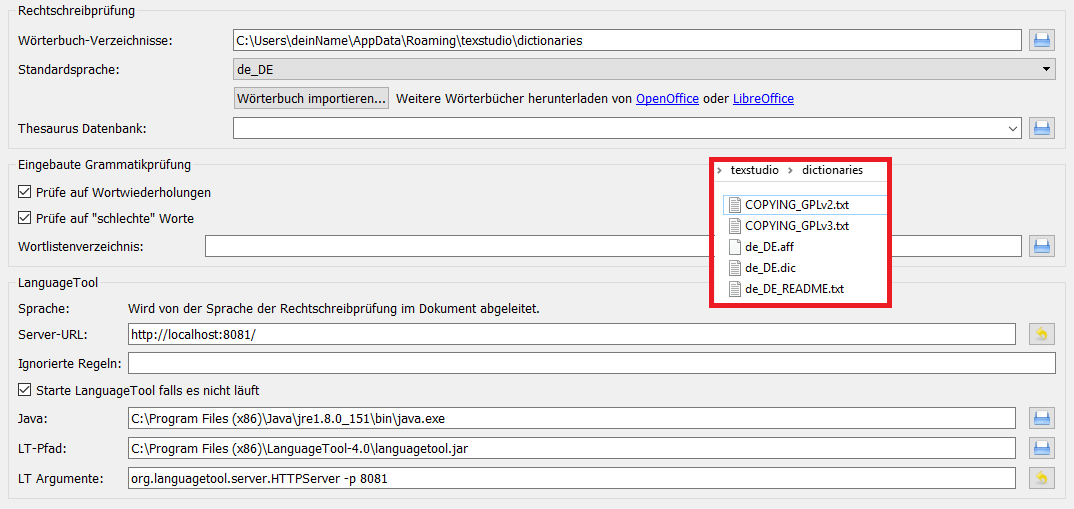
\includegraphics[width=120mm]{./figures/LanguageToolsSetting}%
	\caption{Einrichtung des LanguageTools in TeXstudio}%
	\label{fig:LanguageTool}%
\end{figure}%
\FloatBarrier%
%
Hast du alle oben beschriebenen Schritte erfolgreich hinter dich gebracht, kann es für dich mit LaTeX losgehen!%

\textbf{Info:} Für gemeinsame LaTeX-Projekte an der TUM (z.\,B.~Paper oder Projektberichte) kann die Website \href{https://sharelatex.tum.de}{\textbf{\textit{Sharelatex (sharelatex.tum.de)}}} verwendet werden. Der große Vorteil davon ist, das mehrere Leute gleichzeitig und live an einem Projekt arbeiten können, während eine Versionsverwaltung wie bspw.\,GIT Änderungen immer erst zeitverzögert darstellen kann.%

Neben dem TeXstudio existiert für Word-Fans ein Latex-Editor namens \href{https://www.lyx.org/}{\textbf{Lyx}}, der sich im Handling ähnlich wie Word verhält, jedoch im Hintergrund Latex-Code erzeugt. Es handelt sich also um einen sogenannten WYSIWYG-Editor (\gls{wysiwyg}), mit dessen Hilfe der Einstieg zu Beginn etwas leichter fällt. Großer Nachteil davon ist allerdings, dass der Lerneffekt hinsichtlich Latex sowie das Verständnis der Zusammenhänge deutlich zurückbleibt und damit Phänomene auftauchen, bei denen nicht verstanden wird, warum das so geschieht. Aus diesem Grund raten wir von der Verwendung eines \gls{wysiwyg}-Editors ab und empfehlen die Kombination aus dem TeXstudio und dieser Anleitung.%
%
%
%
%
%
%
%%%%%%%%%%%%%%%%%%%%%%%%%%%%%%%%%%%%%%%%%%%%%%%%%%%%%%%%
\section{Literaturverwaltung}%
\label{sec:Literaturverwaltung}%
Literaturverwaltungsprogramme oder Referenzmanager helfen bei der Erstellung einer wissenschaftlichen Arbeit, die eigene Literatur zu verwalten und so, auch bei vielen Quellen, den Überblick zu behalten. Beispielsweise können Quellen nach Schlagwörtern geordnet und durchsucht sowie direkt aus dem Programm geöffnet werden. Gleichzeitig können Bibliographien exportiert werden, um sie in das \LaTeX{}-Dokument einzubinden (\FTMfullref{subsec:BibliographieEinbinden}). Einen Überblick über die verschiedenen Literaturverwaltungsprogramme, sowie deren Vor- und Nachteile findest du auf der \href{https://mediatum.ub.tum.de/1316333}{Homepage der Universitätsbibliothek} \cite{Literaturverwaltungsprogramme}.%

Im Rahmen der Campuslizenz wird \href{https://www.ub.tum.de/citavi}{\textit{Citavi}} von der Universitätsbibliothek zur Verfügung gestellt \cite{CitaviCampusLizenz}, weshalb sich die folgenden Beispiele auf \textit{Citavi} beziehen. Auf \textit{macOS} können Programme wie \textit{Mendeley}, \textit{JabRef} oder \textit{BibDesk} genutzt werden.%

Neue Titel (neue Quellen) können als unterschiedliche Typen angelegt werden. Der Typ steuert die möglichen Felder des Eintrags und definiert den Stil der Ausgabe im Literaturverzeichnis des Dokuments. Online"=Quellen sollten als \textit{Internetdokument} angelegt werden. Zudem sollte das Feld \textit{Zuletzt geprüft am} ausgefüllt werden, da dieses im Literaturverzeichnis das Abrufdatum definiert.%

Hilfreiche Tools sind der \textit{Citavi Picker} \cite{CitaviPicker} und der \textit{Mendeley Web Importer} \cite{MendeleyWebImporter}, die in allen gängigen Webbrowsern installiert und genutzt werden können. Sie ermöglichen es, auf den meisten Online"=Literatursammlungen die Quelleninformationen direkt in das Literaturverwaltungsprogramm zu importieren. Gleiches funktioniert mit \textit{RefMan}-Einträgen, die mit \textit{Google Scholar} erstellt und in die Literaturverwaltungsprogramme importiert werden können \cites{Citavi2GoogleScholar}.%
%
%
%
%
%
%%%%%%%%%%%%%%%%%%%%%%%%%%%%%%%%%%%%%%%%%%%%%%%%%%%%%%%%
\section{Grafikprogramme}%
\label{sec:Grafikprogramme}%
Die folgenden Tools eignen sich zum Erstellen verschiedener Arten von Grafiken. Achte immer darauf, eine editierbare Datei zu speichern und wenn möglich ausschließlich Vektorgrafiken zu nutzen! Vektorgrafiken verpixeln nicht und halten die Datei klein.%
\begin{enumerate}%
	\item \href{https://inkscape.org/de/}{\textbf{Inkscape}}: Umfangreiches Programm zur Erstellung und Bearbeitung von Vektorgrafiken.%
	\item \href{https://www.yworks.com/products/yed}{\textbf{yEd Graph}}: Spezialisiert auf Diagramme wie Flowcharts, Klassendiagramme, Mindmaps und viele mehr.%
	\item \href{https://www.draw.io/}{\textbf{draw.io}}: Leicht zu bedienendes Web-Tool zur Erstellung von Diagrammen und Vektorgrafiken.%
	\item \href{https://www.mathcha.io/editor}{\textbf{Mathcha.io}}: Online-Editor zur Erstellung von Formeln und TikZ-Grafiken (u.\,a. Rechtecke, Kreise, Achsen, etc.) nach dem \gls{wysiwyg}-Prinzip. Die Export-Funktion für LaTeX- und TikZ-Code ist ohne Anmeldung verfügbar, mit einem Account können die erstellten Formeln und Grafiken gespeichert und später weiter bearbeitet werden.%
	\item \href{https://code.google.com/archive/p/tikzedt/}{\textbf{Tikzedt}}: Graphischer Editor zur Erstellung von Tikz-Grafiken. Es handelt sich dabei um einen \gls{wysiwyg}-Editor, der auch ohne Installation funktioniert.%
	\item \href{http://www.jonathanleroux.org/software/iguanatex/}{\textbf{IguanaTex}}: Extension für PowerPoint, um Tikz-Umgebungen (wie bspw.~Formeln oder Prinzipskizzen aus Tikz) als Vektor- oder Rastergrafik auf Präsentationsfolien einzubinden. Damit kann der Präsentation in PowerPoint der letzte Schliff gegeben werden und Formeln und Bilder einfach übernommen werden, wenn die schriftliche Ausarbeitung in LaTeX geschrieben wurde.%
\end{enumerate}%
Vektorgrafiken können auch direkt in LaTeX mit Hilfe von TikZ bzw. PGF erstellt werden. Es lassen sich auch MATLAB-Grafiken in TikZ umwanden. Eine detaillierte Beschreibung findest du in \FTMfullref{sec:GrafikenTabellen}.%
%
%
%
%
%
%
%
%%%%%%%%%%%%%%%%%%%%%%%%%%%%%%%%%%%%%%%%%%%%%%%%%%%%%%%%
\section{Produktivität}%
\label{sec:Produktivität}%
\begin{enumerate}%
	\item \href{https://trello.com/}{\textbf{Trello}}: Übersichtliches Tool um Projekte zu organisieren und Aufgaben zu tracken.
	\item \href{https://de.todoist.com/}{\textbf{Todoist}}:	Klassische To-do-Liste mit der Möglichkeit Fristen und Prioritäten hinzuzufügen. %
	\item \href{https://de.atlassian.com/software/confluence}{\textbf{Confluence}}: Umfangreiches Projektmanagement-Tool, bei dem mehrere Benutzer gleichzeitig Dokumente bearbeiten können.%
	\item \href{https://www.gitkraken.com/}{\textbf{Git Kraken}}: Bietet GUI für alle nötigen GIT Funktionen.%
	\item \href{https://toggl.com/}{\textbf{Toggl}}: Zeiterfassungstool mit schneller Bedienung und Zuweisung von Einzel-Projekten und detaillierte wöchentliche und monatliche Auswertungen.%
	\item \href{https://my.timesheet.io/login}{\textbf{Timesheet}}: Detailliertes Zeiterfassungstool mit schneller Bedienung.%
	\item \href{https://autohotkey.com/}{\textbf{Autohotkey}}: Programm zur Erstellung globaler Shortcuts im Betriebssystem, um bspw.~Textbausteine wie neue Tabellen- oder Bild-Umgebungen im Latex-Code zu definieren und somit weniger Tippaufwand zu haben.%
\end{enumerate}%
%
%
%
%
%
%%%%%%%%%%%%%%%%%%%%%%%%%%%%%%%%%%%%%%%%%%%%%%%%%%%%%%%%
\chapter{Aufbau der FTM-Latex-Vorlage}%
\label{chap:Aufbau}%
Die \LaTeX"=Vorlage besteht aus zwei Dateien und zwei Unterordnern.
\begin{itemize}
	\item Die Datei \textit{FTMlatex.cls} ist die sogenannte Dokumenten-Klasse und definiert das Layout und alle wichtigen Definitionen. Sie darf nicht verändert werden!%
	\item Die Datei \textit{main.tex} ist die Hauptdatei, die alle weiteren Dokumente inkludiert und den Aufbau des Dokuments steuert.%
	\item Der Unterordner \textit{figures} ist für alle Arten von Grafikdatei gedacht, die im Dokument genutzt werden. Der Pfad zum Unterordner ist als Standard"=Grafikpfad definiert (\FTMfullref{subsec:GrafikenEinfuegen}).%
	\item Der Unterordner \textit{source} ist für alle weiteren \LaTeX{}-Dateien gedacht, wie beispielsweise die Abkürzungsliste, die Kapitel oder die eigenen Erweiterungen.%
	\item Ist ein Package noch nicht definiert oder sollen eigene Makros, Befehle etc. definiert werden, so sollte dies in \textit{source/your\_own\_definitions} geschehen.%
\end{itemize}%
%
%
%
%
%
%%%%%%%%%%%%%%%%%%%%%%%%%%%%%%%%%%%%%%%%%%%%%%%%%%%%%%%%
\chapter{Arbeiten mit der FTM-Latex-Vorlage}%
\label{chap:Arbeiten}%
In diesem Kapitel wird beschrieben, wie die wichtigsten Elemente einer wissenschaftlichen Arbeit, wie beispielsweise das Literaturverzeichnis, Grafiken oder Tabellen, in \LaTeX{} erstellt werden. Zudem werden einige hilfreiche Tipps und Tricks sowie Bug-Fixes vorgestellt.%
\FTMinstruction{Schreiben auf Englisch:}{Grundsätzlich sollen Arbeiten am Lehrstuhl auf Deutsch geschrieben werden. Falls Prof.~Lienkamp dennoch zugestimmt hat, dass die Arbeit auf Englisch verfasst werden darf, kann die Vorlage mithilfe der Option \textit{optEnglish} in der main-Datei (beim Einbinden der Klasse) umgestellt werden.\\%
\textbf{Wichtige Info:} Die Geheimhaltungsverpflichtung und Erklärung müssen auch bei englischen Arbeiten auf Deutsch in die Arbeit eingebunden und unterschrieben werden.}%
%
%
%
%
%
%%%%%%%%%%%%%%%%%%%%%%%%%%%%%%%%%%%%%%%%%%%%%%%%%%%%%%%%
\section{Druck}
\label{sec:Druck}
Für den Druck sollte die Option \textit{optCMYK} der Klasse aktiviert werden. So erkennt der Druckertreiber reine Textseiten als schwarz-weiß und es kann Geld gespart werden.
%
%
%
%
%
%%%%%%%%%%%%%%%%%%%%%%%%%%%%%%%%%%%%%%%%%%%%%%%%%%%%%%%%
\section{Einbinden der Bibliographie und Zitation}%
\label{sec:Zitation}%
Um die Literatursammlung in \LaTeX{} zitieren zu können, muss diese zunächst exportiert und anschließend eingebunden werden. Die einzelnen Schritte und Einstellungen sowie die Zitation werden im Folgenden beschrieben.%
%
%
\subsection{Konfiguration des Bibliographie Prozessors}%
\label{subsec:Bibliographieprozessor}%
Für das korrekte Erzeugen des Literaturverzeichnisses im PDF-Dokument muss der Standard Bibliographie Prozessor, der als Interface zwischen Latex und der Bibliographie-Datei dient, korrekt eingestellt werden. Für die Lehrstuhlvorlage wird \textit{biber} benötigt.%
\FTMinstruction{Auswahl von biber in TeXstudio:}{\textit{Optionen} $\rightarrow$ \textit{TeXstudio konfigurieren...} $\rightarrow$ \textit{Erzeugen} $\rightarrow$ \textit{Standard Bibliographieprogramm} $\rightarrow$ \textit{Biber}}%
\FTMinstruction{Auswahl von biber in TeXmaker (Alternativ):}{\textit{Optionen} $\rightarrow$ \textit{Texmaker konfigurieren...} $\rightarrow$ \textit{Befehle} $\rightarrow$ \textit{Bib(la)tex} $\rightarrow$ \textit{biber \%}}%
%
%
\subsection{Erstellen und Einbinden der Bibliographie}%
\label{subsec:BibliographieEinbinden}%
Zur automatischen Erstellung eines Literaturverzeichnisses müssen die Informationen und Daten der einzelnen Quellen in Latex eingebunden werden. Dies kann entweder direkt im Dokument oder besser über eine Bibliographie-Datei (.bib) geschehen. Erstellt werden können die Bibliographie-Datein aus allen gängigen Literaturverwaltungsprogrammen wie \textit{Citavi} oder \textit{Mendeley}. Für Citavi kann der vordefinierte Exportfilter \textit{FTM.CitaviTX} genutzt werden.%
%
\FTMinstruction{Exportfilter zu \textit{Citavi} hinzufügen:}{Die Datei \textit{FTM.CitaviTX} in \path{C:\Users\<Benutzername>\Dokumente\Citavi<Version>\Settings\Mappings} oder entsprechenden Ordner kopieren (Citavi 6: \path{C:\Users\<Benutzername>\AppData\Local\Swiss Academic Software\Citavi 6\Settings\Mappings}}
%
\FTMinstruction{In \textit{Citavi} erfolgt der Export über:}{\textit{Datei} $\rightarrow$ \textit{Exportieren} $\rightarrow$ \textit{Alle ... Titel in diesem Projekt} $\rightarrow$ \textit{Weiter} $\rightarrow$ \textit{Exportfilter hinzufügen} $\rightarrow$ \textit{FTM} auswählen $\rightarrow$ \textit{Hinzufügen} $\rightarrow$ \textit{FTM} auswählen $\rightarrow$ \textit{Weiter} $\rightarrow$ \textit{Eine Textdatei erstellen} und die Optionen \textit{LaTeX"=Notation verwenden} aktivieren, \textit{URL"=Package verwenden} deaktivieren $\rightarrow$ \textit{Weiter (ggf. als Standard-Einstellung speichern)} $\rightarrow$ \textit{Weiter}}%
%

\FTMtabref{tab:Literaturtypen} zeigt eine Übersicht über die in der Vorlage unterstützten Literaturtypen, sowie die in Citavi zu befüllenden Felder. Zudem werden \textit{DOI}, \textit{ISBN}, \textit{E-Print} Nummern und die \textit{URL} ausgegeben, falls vorhanden. \cites{Test.norm}{Test.patent}{Test.article}{Test.online}{Test.thesis}{Test.report}{Test.book}{Test.inproceedings}{Test.incollection}{Test.collections}{Test.notice}%

\begin{table}[!htbp]%
	\caption{Unterstütze Literaturtypen}%
	\begin{tabular}{M{3cm}|M{3cm} M{2cm} M{5cm}}%
		\toprule%
		\textbf{Literaturtyp}&\multirow{2}{*}{\textbf{Citavi"=Feld}}&\multirow{2}{*}{\textbf{BibTex"=Feld}}&\multirow{2}{*}{\textbf{Beschreibung}}\\%
		\textbf{(BibTeX-Typ)}&&&\\%
		\midrule%
		\multirow{4}{*}{\parbox{3cm}{\centering Norm\\(norm)}} & Titel & title & Name der Norm\\%
		& Normtyp & type & ... \\%
		& Nummer & number & ... \\%
		& Ausgabedatum & date & nur das Jahr wird genutzt\\%
		\midrule%
		\multirow{5}{*}{\parbox{3cm}{\centering Patente\\(patent)}} & Author & author & Erfinder\\%
		& Titel & title & Name des Patents \\%
		& Publikationsland & address  & Land der Publikation\\%
		& Veröffentlichungs-Nr. & number & ...\\%
		& Publikationsdatum & date & ...\\%
		\midrule%
		\multirow{8}{*}{\parbox{3cm}{\centering Zeitschriftenaufsatz\\(article)}} & Author & author & ...\\%
		& Titel & title & Titel: Untertitel \\%
		& Titelzusatz & titleaddon  & ...\\%
		& Zeitschrift & journal & ...\\%
		& Jahrgang & volume & ...\\%
		& Heftnummer & number & ...\\%
		& Seiten von-bis & pages & ...\\%
		& Jahr & year & ...\\%
		\midrule%
		\multirow{6}{*}{\parbox{3cm}{\centering Internetdokument\\(online)}} & Author & author & ...\\%
		& Titel & title & Titel: Untertitel \\%
		& Titelzusatz & titleaddon  & ...\\%
		& Jahr & year & ...\\%
		& Online"=Adresse & url & ...\\%
		& Zuletzt geprüft am & date & ...\\%
		\midrule%
		\multirow{7}{*}{\parbox{3cm}{\centering Hochschulschrift\\(thesis)}} & Author & author & ...\\%
		& Titel & title & Titel: Untertitel \\%
		& Art der Schrift & type  & Dissertation, Master's Thesis, etc.\\%
		& Institution & publisher & ...\\%
		& Hochschule & school & ...\\%
		& Hochschulort & address & ...\\%
		& Datum/Jahr & date & ...\\%
		\midrule%
		\multirow{7}{*}{\parbox{3cm}{\centering Graue Literatur \\ Bericht \\ Report \\(report)}} & Author & author & ...\\%
		& Titel & title & Titel: Untertitel \\%
		& Institution  & institution & ...\\%
		& Erscheinungsort & address & ...\\%
		& Nummer & number & Nummer des Repositoriums\\%
		& Seiten & pages & ...\\%
		& Datum/Jahr & date & Kann auch nur ein Jahr sein\\%
		\midrule%
		\multirow{8}{*}{\parbox{3cm}{\centering Buch (Monographie)\\(book)}} & Author & author & ...\\%
		& Titel & title & Titel: Untertitel \\%
		& Institution  & series & ...\\%
		& Bandnr. der Reihe & volume & ...\\%
		& Auflage & edition & ... \\%
		& Verlag & publisher & ...\\%
		& Seiten & pages & ...\\%
		& Jahr & year & ...\\%
		\midrule%
		\multirow{4}{*}{\parbox{3cm}{\centering Beitrag\\in Tagungsband\\(inproceedings)}} & Author & author & ...\\%
		& Titel & title & Titel: Untertitel \\%
		& Seiten & pages & ...\\%
		& Jahr & year & ...\\%
		\multirow{2}{*}{\parbox{3cm}{\centering Tagungsband\\(proceedings)}} & Titel & title & Titel: Untertitel (Tagungsband) \\%
		& Tagungsort & venue & ... \\%
		\midrule%
	\end{tabular}%
	\label{tab:Literaturtypen}%
\end{table}%
\begin{table}[!htbp]%
	\begin{tabular}{M{3cm}|M{3cm} M{2cm} M{5cm}}%
		\midrule%
		\multirow{4}{*}{\parbox{3cm}{\centering Beitrag\\in Sammelwerk\\(incollection)}} & Author & author & ...\\%
		& Titel & title & Titel: Untertitel \\%
		& Bandnummer & volume & ...\\%
		& Seiten & pages & ...\\%
		\multirow{6}{*}{\parbox{3cm}{\centering Sammelwerk\\(collection)}} & Titel & title & Titel: Untertitel (Sammelwerk) \\%
		& Herausgeber & editor & ... \\%
		& Reihentitel & series & ... \\%
		& Verlag & publisher & ... \\%
		& Verlagsort & address & ... \\%
		& Jahr & year & ...\\%
		\midrule%
		\multirow{6}{*}{\parbox{3cm}{\centering Persönliche Mitteilung\\(notice)}} & Titel & title & Titel: Untertitel (Sammelwerk) \\%
		& Titelzusatz & titleaddon  & ...\\%
		& Author & author & ...\\%
		& Mitteilungsform & type  & ...\\%
		& Datum & date & ... \\%
		\bottomrule%
	\end{tabular}%
\end{table}%
Dissertationen und Studienarbeiten müssen als \textit{Hochschulschrift}  angelegt werden, unter \textit{Art der Schrift (Type)} kann dann die Art der Arbeit angegeben werden.%

Nutzer anderer Literaturverwaltungsprogramme müssen sich den Exportfilter entsprechend der Übersicht in Anhang \FTMtabref{tab:Literaturtypen} erstellen.%

In der Lehrstuhlvorlage wird die Datei \textit{./source/literature.bib} eingebunden. Diese Datei muss mit der eignen Bibliographie ersetzt werden.%
\FTMinstruction{Einbinden der Bibliographie in die Vorlage:}{In der Vorlage muss die Datei \textit{./source/literature.bib} mit der eigenen Bibliographie ersetzte werden (ggf. Dateinamen in der main.tex anpassen)}%
%
%
\subsection{Definition eigener Cite-Keys}%
\label{subsec:Cite-Key}%
Die erstellte Bibliographie-Datei (\FTMsecref{subsec:BibliographieEinbinden}) enthält alle Informationen über die jeweilige Quelle, die in der Literaturverwaltung hinterlegt sind. Beim Export wird zudem ein sogenannter \textit{Key} erstellt, über den die jeweilige Quelle in Latex zitiert werden kann. Der \textit{Key} in Zeile 1 von \FTMlstref{lst:Bibliographie} wird standardmäßig aus Autor.Jahr erstellt.%

\begin{minipage}{\linewidth}%
\begin{lstlisting}[language=tex, caption=Auszug einer Bibliographie-Datei,label=lst:Bibliographie]
@book{Lienkamp.2013,
 author = {Lienkamp, Markus},
 year = {2013},
 title = {Conference on Future Automotive Technology: Focus Electro Mobility},
 url = {http://dx.doi.org/10.1007/978-3-658-01141-3},
 address = {Wiesbaden},
 publisher = {{Springer Fachmedien Wiesbaden}},
 isbn = {978-3-658-01141-3}}
\end{lstlisting}%
\end{minipage}%

Zur manuellen Verwaltung der \textit{Keys} kann dieser in den meisten Literaturverwaltungsprogrammen manuell angegeben werden.%
\FTMinstruction{BibTex Key Erweiterung in Citavi aktivieren:}{\textit{Extras} $\rightarrow$ \textit{Optionen...} $\rightarrow$  TeX-Unterstützung aktivieren $\rightarrow$ \textit{OK}\newline Anschließend erscheint im Reiter \textit{Titel} ein neues Feld \textit{BibTeX Key}}%
%
\subsection{Zitieren}%
\label{subsec:Zitieren}%
Ein Zitat kann in Latex mit Hilfe des Befehls \verb|\cite{}|, beziehungsweise \verb|\cites{}{}| für mehrere Quellen in einem Zitat, angegeben werden. Die Auflistung der Quelle im Literaturverzeichnis erfolgt anschließend automatisch in der Reihenfolge der Zitationen.\\%
Als Parameter wird in geschweiften Klammern der \textit{Key} der jeweiligen Quelle übergeben, wie er in der Bibliographie-Datei (\textit{literatur.bib}) definiert ist. Als optionaler Parameter kann in eckigen Klammern vor der Quelle zusätzlich eine Seitenzahl oder ein Kapitel angegeben werden.%

\textbf{Beispiel}: Die Frage ob Elektromobilität ein Hype oder eine Revolution ist stellt auch Lienkamp \cite{L12Hype}.%
\begin{lstlisting}[language=tex, caption=Zitieren einer Quelle ohne Seitenangaben]
\cite{Lienkamp.2012}
\end{lstlisting}%
Es können auch mehrere Zitate zusammengefügt werden \cites[S.\,5f]{Me1}[S.\,5-15]{studentsThesis1} oder \cite{Me1,studentsThesis1,FTM}.%
\begin{lstlisting}[language=tex, caption=Zitieren mehrerer Quellen (inklusive Seitenangaben)]
\cites[S.\,5f]{Me1}[S.\,5-15]{studentsThesis1}
\cites{Me1,studentsThesis1,FTM}
\end{lstlisting}%
Der Befehlt \verb|\,| stellt ein halbes geschütztes Leerzeichen sicher (\FTMsecref{sec:SonderzeichenUndSilbentrennung}).%

Um für Online-Quellen im Literaturverzeichnis das Datum des Abrufs an den Eintrag anzufügen, muss in der Bibliographie im Feld \textit{urldate} bzw. in Citavi im Feld \textit{Zuletzt geprüft am} das Datum des Seitenaufrufs angegeben werden \cite{FTM}.%

Zur korrekten Darstellung von Eigennamen, ist der Befehlt \verb|\relax{}| hilfreich.%
\begin{lstlisting}[language=tex, caption=Eigennamen im Literaturverzeichnis korrekt darstellen]
Author = {\relax{Lehrstuhl für Fahrzeugtechnik München}}
\end{lstlisting}%
Weitere Details zum Thema Zitieren sind online zu finden. \cite{citePackage}%
%
%
\subsection{Aufbau des Literaturverzeichnisses}%
\label{subsec:Literaturverzeichnis}%
Das Literaturverzeichnis listet alle im Text zitierten Quellen in der Reihenfolge der Zitation. Der Zitationsstil richtet sich dabei nach der Art der Quelle, wie beispielsweise \textit{article}, \textit{online} oder \textit{misc}.Der Zitationsstil und das Layout der Zitate wird in der Klasse \textit{FTMLatex.cls} definiert und darf nicht verändert werden%
\subsubsection{Erweitertes Literaturverzeichnis}%
\label{subsubsec:ErweitertesLiteraturverzeichnis}%
Das erweiterte Literaturverzeichnis ist für Dissertationen vorgesehen und besteht aus zwei Teilen. Dem vollständigen Literaturverzeichnis der Arbeit und den Vorveröffentlichungen inklusive der studentischen Arbeiten. In Studienarbeiten gibt es nur die Erweiterung Eigene Veröffentlichungen. In welchen Verzeichnissen eine Quelle erscheint, kann mithilfe der folgenden Keywords im Literaturverwaltungsprogramm gesteuert werden:
 \begin{table}[!htbp]
	\begin{tabularx}{0.85\textwidth}{M{0.2\textwidth} p{0.6\textwidth}}
		\toprule
		\textbf{Keyword}&\textbf{Erklärung}\\
		\midrule
		me & eigene Veröffentlichung\\
		peerReview & Veröffentlichung ist peer-reviewed (nur in Verbindung mit me)\\
		\multirow{2}{*}{nonRelevant} & Veröffentlichung ist peer-reviewed aber nicht relevant für die Dissertation (nur in Verbindung mit me)\\
		studentsThesis & betreute Studienarbeit\\
		inPress & im Druck aber noch nicht veröffentlicht (nur in Verbindung mit me)\\
		accepted & akzeptiert aber noch nicht im Druck (nur in Verbindung mit me)\\
		inReview & eingereicht aber noch im Review-Prozess (nur in Verbindung mit me)\\
		\bottomrule
	\end{tabularx}
	\caption{Steuerung der Literaturverzeichnisses mittels Key-Word}
	\label{tab:KeyWords}
\end{table}%
\FloatBarrier%
\begin{lstlisting}[language=tex, caption=Auszug einer Bibliographie-Datei mit Keyword,label=lst:BibliographieKeyword]
@phdthesis{studentsThesis1,
Adress = {M{\"u}nchen},
Author = {Eins, Student},
Type = {Bachelor's Thesis},
Keywords = {studentsThesis},
School = {TU M{\"u}nchen},
Title = {Bachelor's Thesis},
Year = {2017}}
\end{lstlisting}%
Alle Einträge, die mithilfe des Befehls \verb|\nocite{}| hinzugefügt werden, werden ohne Nummer in das Literaturverzeichnis angefügt. Wie bei allen Einträgen zählt hier die Reihenfolge der Zitationen im Text. Aus diesem Grund sollten die nicht zitierten Quellen am Ende des Dokuments in sinnvoller Sortierungsreihenfolge (bspw. Autor, Titel, Jahr) hinzugefügt werden.%
%
%
%
%
%
%%%%%%%%%%%%%%%%%%%%%%%%%%%%%%%%%%%%%%%%%%%%%%%%%%%%%%%%
\section{Sonderzeichen und Silbentrennung}%
\label{sec:SonderzeichenUndSilbentrennung}%
Bei \LaTeX{} handelt es sich um eine Programmiersprache, daher ist es nötig, Sonderzeichen \glqq{}maskiert\grqq{} in den \LaTeX"=Editor einzugeben. Die maskierte Eingabe erfolgt über definierte Codes, die \LaTeX{} beim Erstellen des PDFs interpretiert. Zu diesen Codes gehören auch sogenannte Steuerzeichen, mit deren Hilfe die Silbentrennung beeinflusst werden kann. Eine Übersicht der Sonder- und Steuerzeichen findet sich in \FTMtabref{tab:Sonderzeichen}.%
\begin{table}[!htbp]%
	\caption{Sonder- und Steuerzeichen in \LaTeX{}}%
	\begin{tabular}{c c p{8 cm}}%
		\toprule%
		\textbf{Latex-Code}&\textbf{Beispiel}&\textbf{Beschreibung}\\%
		\midrule%
		\verb|\glqq{}| & \glqq{}Test & \textbf{Anführungszeichen unten}\newline%
			\verb|Er sagt: \glqq{}Hallo!\grqq{}|\\%
		\verb|\grqq{}| & Test\grqq{} & \textbf{Anführungszeichen oben}\\%
		\midrule%
		\verb|Ein\,Test| & Ein\,Test & \textbf{Halbes (geschütztes) Leerzeichen}\newline%
			Für Verwendung in Abkürzungen wie bspw. \glqq{}z.\,B.\grqq{}, damit Abstand zwischen Punkt und B passt: \verb|z.\,B.|\\%
		\verb|Ein~Test| & Ein~Test & \textbf{Ganzes geschütztes Leerzeichen}\newline%
			Leerzeichen, das einen Umbruch an dieser Stelle verhindert. Beispielsweise um \glqq{}z.\,B.\grqq{} nicht am Zeilenende stehen zu lassen oder Wert und Einheit nicht zu trennen: \verb|z.\,B.~Testtext| und \verb|10~Prozent|\\%
		\midrule%
		\verb|-| & x - y & \textbf{Bindestrich/ Viertelgeviertstrich} (kurz), Verwendung für Worttrennungen (am Zeilenumbruch), Zusammengesetzte Wörter, Wortergänzungen
		\\%
		\verb|--| & x -- y & \textbf{Bindestrich/ Halbgeviertstrich/ Gedankenstrich} (mittellang), Verwendung für Zahlenbereiche wie bspw.~\glqq{}20\,--\,30\grqq{} in Form von \verb|20\,--\,30|\grqq{}, Zeichen für "gegen" (Bsp: Bayern München -- Borussia Dortmund), Streckenangaben (Bsp: Die Strecke Hamburg -- Hannover -- München) oder als Gedankenstrich.\\%
		\midrule%
		%
		\multicolumn{3}{c}{\textbf{Silbentrennung für Wörter mit Bindestriche (nur für deutsche Vorlage gültig!)}}\\%
		\verb|Silben-Trennung| & Silben-Trennung & \textbf{nur} am Bindestrich darf getrennt werden\\%
		\verb|Silben"=Trennung| & Silben"=Trennung & \textbf{auch} am Bindestrich darf getrennt werden\\%
		\verb|Silben"~Trennung| & Silben"~Trennung & am Bindestrich \textbf{darf nicht} getrennt werden\\%
		%
		\multicolumn{3}{c}{\textbf{Anpassungen der Silbentrennung innerhalb von Wörtern}}\\%
		\multicolumn{3}{c}{\textbf{(nur für deutsche Vorlage gültig!)}}\\%
		\verb|Silben\-trennung| & Silben\-trennung & \textbf{nur} an dieser Trennstelle darf getrennt werden (andere Silbentrennungen werden unterbunden); Verwendung für Haupttrennfugen bei zusammengesetzten Worten, z.\,B.~\verb|Elektro\-fahrzeuge|, um schlecht lesbare Trennungen wie bspw.~Elektrofahr-zeuge zu vermeiden.\\%
		\verb|Silben"-trennung| & Silben"-trennung & \textbf{auch} an dieser Trennstelle darf getrennt werden;\newline%
			Kann verwendet werden, falls \LaTeX{} eine Trennstelle nicht automatisch findet: z.\,B.~\verb|Am"-nestie|\\%
		\verb|Silben""trennung| & Silben""trennung & \textbf{Trennmöglichkeit}, bei der \textbf{kein Trennstrich benötigt} wird\\%
%		\verb|Silben"¦trennung| & Silben"¦trennung & Auflösen einer Ligatur und Schaffung einer Trennmöglichkeit\\% Was auch immer das ist...
		\bottomrule%
	\end{tabular}%
	\label{tab:Sonderzeichen}%
\end{table}%
%
%
%
%
%
%%%%%%%%%%%%%%%%%%%%%%%%%%%%%%%%%%%%%%%%%%%%%%%%%%%%%%%%
\section{Grafiken und Tabellen}%
\label{sec:GrafikenTabellen}%
Grafiken, Abbildungen, Diagramme und Tabellen können genutzte werden, um den Fließtext zu unterbrechen und dem Leser wichtige Inhalte und Informationen auf einem zusätzlichen Informationskanal zu präsentieren. Damit diese auch zu einem besseren Verständnis beitragen, ist es wichtig, stets Fließtext und Grafik oder Tabelle zu verknüpfen und einen Zusammenhang herzustellen.%
%
%
\subsection{Layout von Grafiken und Tabellen}%
\label{subsec:GrafikenLayout}%
Allgemein dürfen Grafiken und Tabellen eine maximale Breite von \SI{90}{\percent} der Textbreite besitzen und sind zentriert. Grafiken werden mit Bildunterschriften, Tabellen mit Überschriften beschriftet. Die Formatierung der Beschriftungen (\textbackslash \textit{caption}) ist in der \LaTeX"=Vorlage bereits definiert.%
%
%
%%%%%%%%%%%%%%%%%%%%%%%%%%%%%%%%%%%%%%%%%%%%%%%%%%%%%%%%
\subsection{TUM-Farben}%
\label{sec:TUM_Farben}%
%
Für Grafiken sollen nach Möglichkeit die offiziellen Farben der TUM nach \FTMtabref{tab:TUM_Farben} verwendet werden. Die Farben sind bereits vordefiniert und können mit den angegebenen Namen (bspw. \verb|TUMBlue|) verwendet werden. Es sollte darauf geachtet werden, dass die Grafiken auch bei DIN A5 drucken in schwarz-weiß noch gut lesbar sind.
%
\begin{table}[!htbp]%
	\begin{tabular}[t]{|l|c|c|c|c|c|c|c|c|c|}%
		\hline%
		\textbf{Color} & \textbf{R} & \textbf{G} & \textbf{B} & \textbf{C} & \textbf{M} & \textbf{Y} & \textbf{K} & \textbf{Hex} & \textbf{Preview} \\\hline\hline%
		TUMBlue & 0 & 101 & 189 & 100 & 43 & 0 & 0 & \texttt{0x0065BD} & \raisebox{-0.25em}{\tikz \fill [TUMBlue] (0,0) rectangle (1.3cm,1em);} \\\hline%
		TUMWhite & 255 & 255 & 255 & 0 & 0 & 0 & 0 & \texttt{0xFFFFFF} & \raisebox{-0.25em}{\tikz \fill [TUMWhite] (0,0) rectangle (1.3cm,1em);} \\\hline%
		TUMBlack & 0 & 0 & 0 & 0 & 0 & 0 & 100 & \texttt{0x000000} & \raisebox{-0.25em}{\tikz \fill [TUMBlack] (0,0) rectangle (1.3cm,1em);} \\\hline%
		%
		TUMBlue1 & 0 & 51 & 89 & 100 & 57 & 12 & 70 & \texttt{0x003359} & \raisebox{-0.25em}{\tikz \fill [TUMBlue1] (0,0) rectangle (1.3cm,1em);} \\\hline%
		TUMBlue2 & 0 & 82 & 147 & 100 & 54 & 4 & 19 & \texttt{0x005293} & \raisebox{-0.25em}{\tikz \fill [TUMBlue2] (0,0) rectangle (1.3cm,1em);} \\\hline%
		TUMGray1 & 51 & 51 & 51 & 0 & 0 & 0 & 80 & \texttt{0x333333} & \raisebox{-0.25em}{\tikz \fill [TUMGray1] (0,0) rectangle (1.3cm,1em);} \\\hline%
		TUMGray2 & 127 & 127 & 127 & 0 & 0 & 0 & 50 & \texttt{0x7F7F7F} & \raisebox{-0.25em}{\tikz \fill [TUMGray2] (0,0) rectangle (1.3cm,1em);} \\\hline%
		TUMGray3 & 204 & 204 & 204 & 0 & 0 & 0 & 20 & \texttt{0xCCCCCC} & \raisebox{-0.25em}{\tikz \fill [TUMGray3] (0,0) rectangle (1.3cm,1em);} \\\hline%
		%
		TUMBlue3 & 100 & 160 & 200 & 65 & 19 & 1 & 4 & \texttt{0x64A0C8} & \raisebox{-0.25em}{\tikz \fill [TUMBlue3] (0,0) rectangle (1.3cm,1em);} \\\hline%
		TUMBlue4 & 152 & 198 & 234 & 42 & 9 & 0 & 0 & \texttt{0x98C6EA} & \raisebox{-0.25em}{\tikz \fill [TUMBlue4] (0,0) rectangle (1.3cm,1em);} \\\hline%
		TUMIvory & 218 & 215 & 203 & 3 & 4 & 14 & 8 & \texttt{0xDAD7CB} & \raisebox{-0.25em}{\tikz \fill [TUMIvory] (0,0) rectangle (1.3cm,1em);} \\\hline%
		TUMOrange & 227 & 114 & 34 & 0 & 65 & 95 & 0 & \texttt{0xE37222} & \raisebox{-0.25em}{\tikz \fill [TUMOrange] (0,0) rectangle (1.3cm,1em);} \\\hline%
		TUMGreen & 162 & 173 & 0 & 35 & 0 & 100 & 20 & \texttt{0xA2AD00} & \raisebox{-0.25em}{\tikz \fill [TUMGreen] (0,0) rectangle (1.3cm,1em);} \\\hline%
	\end{tabular}%
	\caption{Definition der TUM-Farben}
	\label{tab:TUM_Farben}
\end{table}
\FloatBarrier%
%
%
\subsection{Einfügen von Tabellen}%
\label{subsec:Tabellen}%
In Latex gibt es die unterschiedlichsten Environments zum Einfügen von Tabellen, an dieser Stelle wird \textit{tabularx} vorgestellt. Den klassischen Aufbau einer Tabelle zeigt \FTMlstref{lst:table}
\begin{lstlisting}[language=TeX, caption=Einfügen einer Tabelle, label=lst:table]
\begin{table}[<float-Positionierung im Text>]
	\begin{tabularx}{<Breite>}{<Spaltenformatierung>}
		\toprule
			<Spaltenüberschriften>
		\midrule
			<Zeilen und Spalten>
		\bottomrule
	\end{tabularx}
	\caption{<Tabellenüberschrift>}
	label{tab:table}
\end{table}
\end{lstlisting}%
In Zeile 1 wird zunächst ein \textit{table}"=Environment gestartet, das automatisch zentriert ist, innerhalb dessen wiederum ein \textit{tabularx}"=Environment mit der gewünschten Breite und Spaltenformatierung, entsprechend \FTMtabref{tab:Tabellen}, begonnen wird (Zeile 2). Anschließend folgt der Tabelleninhalt (Zeile 3-7), Spalten werden durch \verb|&| getrennt, Zeilen durch \verb|\\|. Bevor das äußere \textit{table}"=Environment geschlossen wird (Zeile 11), muss noch eine Überschrift (Zeile 9) und ein Label (Zeile 10) vergeben werden (Zeile 11).
 \begin{table}[!htbp]
	\begin{tabularx}{0.5\textwidth}{c l}
		\toprule
		\textbf{Option}&\textbf{Erklärung}\\
		\midrule
		X & Spalte mit variabler Breite\\
		c & zentrierte Spalte\\
		l & linksbündige Spalte\\
		r & rechtsbündige Spalte\\
		p\{breite\} & Minipage mit der Breite oben ausgerichtet\\
		m\{breite\} & Minipage mit der Breite mittig ausgerichtet\\
		b\{breite\} & Minipage mit der Breite unten ausgerichtet\\
		$\vert$ & vertikale Trennlinie\\
		\midrule
		\multirow{2}{*}{M\{breite\}} & Minipage mit der Breite mittig ausgerichtet\\
		& und zentriert (eigene Definition)\\
		\bottomrule
	\end{tabularx}
	\caption{Formatierungsoptionen der Spalten im Tabularx"=Package}
	\label{tab:Tabellen}
\end{table}%
\FloatBarrier%
Das Beispiel aus \FTMtabref{tab:Tabellen} zeigt \FTMlstref{lst:TabellenBeispiel}:
\begin{lstlisting}[language=TeX, caption=Beispieltabelle, label=lst:TabellenBeispiel]
\begin{table}[!htbp]
	\begin{tabularx}{0.5\textwidth}{c l}
		\toprule
		\textbf{Option}&\textbf{Erklärung}\\
		\midrule
		X & Spalte mit variabler Breite\\
		c & zentrierte Spalte\\
		l & linksbündige Spalte\\
		r & rechtsbündige Spalte\\
		p\{breite\} & Minipage mit der Breite oben ausgerichtet\\
		m\{breite\} & Minipage mit der Breite mittig ausgerichtet\\
		b\{breite\} & Minipage mit der Breite unten ausgerichtet\\
		$\vert$ & vertikale Trennlinie\\
		\midrule
		\multirow{2}{*}{M\{breite\}} & Minipage mit der Breite mittig ausgerichtet\\
		& und zentriert (eigene Definition)\\
		\bottomrule
	\end{tabularx}
	\caption{Formatierungsoptionen der Spalten im Tabularx"=Package}
	\label{tab:Tabellen}
\end{table}
\end{lstlisting}
Um Spalten oder Zeilen zusammenzuführen gibt es die Möglichkeit
\begin{lstlisting}[language=TeX, caption=Zusammenführen von Zeilen und Spalten in Tabellen, label=lst:multirow]
\multirow{<Anzahl der Reihen>}{<Spaltenbreite>}{<Text>}
\multicolumn{<Anzahl der Spalten>}{<Formatierung>}{<Text>}
\end{lstlisting}%
zu nutzen. Die Dokumentation des \textit{tabularx}"=Packages \cite{tabularxDocumentation} und des \textit{multirow}"=Packages \cite{multirowDocumentation}  findet man wie viele weitere Dokumentationen im Rahmen des \gls{ctan}.
%
%
\subsection{Einfügen von Grafiken}%
\label{subsec:GrafikenEinfuegen}%
In Latex können die verschiedensten Dateiformate für Grafiken eingefügt werden. Zum Einbinden muss zunächst eine Bildumgebung (Zeile 1 und 6) erstellt werden, die automatisch zentriert ist. Die Grafik wird in Zeile 2 eingefügt, in Zeile 3 die Bildunterschrift und in Zeile 4 das Label zum Referenzieren definiert.%
\begin{lstlisting}[language=TeX, caption={Einfügen einer Grafik mittels figure-Umgebung und hier noch eine etwas längere Überschrift um zu zeigen, wie die hang-Formatierung die Beschriftung umbricht}, label=lst:Figure]
\begin{figure}[!htbp]
	
\includegraphics[width=40mm]{./ImagePNG}
	\caption[PNG-Grafik]{Das ist eine PNG-Grafik}
	\label{fig:pngGrafik}
\end{figure}
\end{lstlisting}%
Das Ergebnis aus \FTMlstref{lst:Figure} zeigt \FTMfigref{fig:pngGrafik}:
\begin{figure}[!htbp]
	
\includegraphics[width=40mm]{./ImagePNG}
	\caption[PNG-Grafik]{Das ist eine PNG-Grafik und auch hier wollen wir mal schauen, wie sich die Einstellung verhält, wenn die Bildunterschrift in die zweite Zeile umbricht}
	\label{fig:pngGrafik}
\end{figure}%
Die Bildunterschrift für das Abbildungsverzeichnis kann getrennt definiert werden, wenn zum Beispiel Simulationsparameter weggelassen oder zu lange Unterschriften gekürzt werden sollen. Die Definition erfolgt wie in Zeile 4 von \FTMlstref{lst:Figure} in eckigen Klammern.%

Abbildungen, die sich aus mehreren Einzelabbildungen zusammensetzen, können mit Hilfe des \textit{subcpation}-Packages erstellt werden. Dabei sollte für jede Einzelabbildung eine Beschriftung hinzugefügt und ein Label definiert werden.%

\begin{lstlisting}[language=tex, caption=Zusammengesetzte Abbildung aus mehreren Einzelabbildungen, label=lst:Subfigure]
\begin{figure}[!htbp]
\begin{subfigure}[t]{0.3\textwidth}%
	\centering%
	\begin{tikzpicture}
\draw[draw=black, line width=1pt] (0,0) rectangle (4,4);
\node[anchor=center] at (2,2) {\Large A};
\end{tikzpicture}%%
	\subcaption{Bild a hat eine etwas längere Bildunterschrift um zu testen, ob die Option \textit{hang} funktioniert}%
	\label{fig:subfig_a}%
\end{subfigure}\quad%
\begin{subfigure}[t]{0.3\textwidth}%
	\centering%
	\input{./figures/Tikz_Subfig_b}%
	\subcaption{Bild b}%
	\label{fig:subfig_b}%
\end{subfigure}\par\bigskip%
\begin{subfigure}[t]{0.3\textwidth}%
	\centering%
	\input{./figures/Tikz_Subfig_c}%
	\subcaption{Bild c}%
	\label{fig:subfig_c}%
\end{subfigure}\quad%
\begin{subfigure}[t]{0.3\textwidth}%
	\centering%
	\input{./figures/Tikz_Subfig_d}%
	\subcaption{Bild d}%
	\label{fig:subfig_d}%
\end{subfigure}%
\caption{Dieses Bild wurde mit dem subcaption-Package erstellt}
   \label{fig:subfig}
\end{figure}%
\end{lstlisting}%
\begin{figure}[!htbp]
\begin{subfigure}[t]{0.3\textwidth}%
	\centering%
	\begin{tikzpicture}
\draw[draw=black, line width=1pt] (0,0) rectangle (4,4);
\node[anchor=center] at (2,2) {\Large A};
\end{tikzpicture}%%
	\subcaption{Bild a hat eine etwas längere Bildunterschrift um zu testen, ob die Option \textit{hang} funktioniert}%
	\label{fig:subfig_a}%
\end{subfigure}\quad%
\begin{subfigure}[t]{0.3\textwidth}%
	\centering%
	\input{./figures/Tikz_Subfig_b}%
	\subcaption{Bild b}%
	\label{fig:subfig_b}%
\end{subfigure}\par\bigskip%
\begin{subfigure}[t]{0.3\textwidth}%
	\centering%
	\input{./figures/Tikz_Subfig_c}%
	\subcaption{Bild c}%
	\label{fig:subfig_c}%
\end{subfigure}\quad%
\begin{subfigure}[t]{0.3\textwidth}%
	\centering%
	\input{./figures/Tikz_Subfig_d}%
	\subcaption{Bild d}%
	\label{fig:subfig_d}%
\end{subfigure}%
\caption{Dieses Bild wurde mit dem subcaption-Package erstellt}
   \label{fig:subfig}
\end{figure}%

Durch die Definition von Labels für jede der Einzelabbildungen kann entweder die gesamte \FTMfigref{fig:subfig} oder jede einzelne \FTMfigtoref{fig:subfig_a}{fig:subfig_d} referenziert werden (\FTMsecref{sec:Referenzieren}).%

Der Unterordner \textit{figures} wird in der Vorlage als Standard-Grafikpfad definiert, weshalb Grafiken in diesem Ordner mit Hilfe von \verb|\includegraphics| ohne relativen Pfad eingefügt werden können.%

Das gleiche funktioniert auch mit Tabellen. Hierfür muss ein \textit{table}-Environment genutzt werden. Um die Captions über die Tabelle zu bekommen, muss der \textit{subcaption}-Befehl im \textit{subtable}-Environment vor der Tabelle stehen. Da sich die \textit{subtable} und \textit{subfigure} Environments wie \textit{minipages} verhalten, sind die Breitenangaben innerhalb der Environments relativ auf die Breitenangaben der Environments bezogen.

\begin{table}[!htbp]
\begin{subtable}[t]{0.4\textwidth}%
	\centering%
	\subcaption{Tabelle a}%
	\begin{tabularx}{0.7\textwidth}{c l}%
		\toprule%
		\textbf{Spalte 1}&\textbf{Spalte 2}\\%
		\midrule%
		1 & Alpha\\%
		2 & Beta\\%
		\bottomrule%
	\end{tabularx}%
\end{subtable}\quad%
\begin{subtable}[t]{0.4\textwidth}%
	\centering%
	\subcaption{Tabelle b}%
	\begin{tabularx}{0.7\textwidth}{c l}%
		\toprule%
		\textbf{Spalte 1}&\textbf{Spalte 2}\\%
		\midrule%
		3 & Gamma\\%
		4 & Delta\\%
		\bottomrule%
	\end{tabularx}%
\end{subtable}\par\bigskip %
\begin{subtable}[t]{0.4\textwidth}%
	\centering%
	\subcaption{Tabelle c}%
	\begin{tabularx}{0.7\textwidth}{c l}%
		\toprule%
		\textbf{Spalte 1}&\textbf{Spalte 2}\\%
		\midrule%
		5 & Epsion\\%
		6 & Zeta\\%
		\bottomrule
	\end{tabularx}%
\end{subtable}\quad%
\begin{subtable}[t]{0.4\textwidth}%
	\centering%
	\subcaption{Tabelle d}%
	\begin{tabularx}{0.7\textwidth}{c l}%
		\toprule%
		\textbf{Spalte 1}&\textbf{Spalte 2}\\%
		\midrule%
		7 & Eta\\%
		8 & Theta\\%
		\bottomrule%
	\end{tabularx}%
\end{subtable}\\%
\caption{Diese Mehrfach-Tabelle wurde mit dem subcaption-Package erstellt}
   \label{fig:subtab}
\end{table}%

%
%
\subsection{Platzieren von Grafiken und Tabellen}
\label{subsec:GrafikenPlatzieren}
Grafiken und Tabellen werden mit Hilfe des \textit{Float}-Environments platziert. Je nach Reihenfolge und Auswahl der Ausrichtungsoptionen hinter der Grafik oder Tabellendefinition (\FTMlstref{lst:Figure} und \FTMlstref{lst:TabellenBeispiel} Zeile 1) wird die Grafik im Text positioniert.%
\begin{table}[!htbp]
	\begin{tabularx}{0.6\textwidth}{c l}
		\toprule
		\textbf{Option}&\textbf{Positionierung}\\
		\midrule
		h & hier\\%
		t & Seitenanfang\\%
		b & Seitenende\\%
		p & extra Seite\\%
		! & Parameter für bessere Positionierung überschreiben\\%
		H & genau hier (nicht empfohlen)\\%
		!htbp & Empfohlene Einstellung\\%
		\bottomrule
	\end{tabularx}
	\caption{Positionierung von Float-Objekten, auch hier wollen wir schauen, wie es sich verhält, wenn die Tabellenüberschrift in die nächste Zeile umbricht}
	\label{tab:Float}
\end{table}%
\FloatBarrier%
Es wird die Einstellung \verb|!htbp| empfohlen. Mit dem Befehl \verb|\FloatBarrier| kann eine untere Grenze definiert werden, bis zu der alle zuvor definierten Float-Objekt positioniert werden müssen. Statt \verb|H| sollte besser eine \verb|\FloatBarrier| direkt hinter dem Objekt genutzt werden. Um leere Zeilen an das Ende eines Kapitels bzw. einer Seite zu schieben, kann der Befehl \verb|\vfill| genutzt werden.%
%
%
\subsection{Vektorgrafiken}%
\label{subsec:Vektorgrafiken}
Grafikformaten wie \textit{.jpg} oder \textit{.png} sind sogenannte Rastergrafiken, die jedem Pixel einen Farbwert zuweisen. Das hat zur Folge, dass detailreiche Grafiken entweder verpixelt wirken oder die Datei sehr groß wird. Dies führt wiederum zu einem unschönen Erscheinungsbild oder einer großen PDF-Datei. Im Gegensatz dazu speichern Vektorgrafiken Formparameter wie Kreismittelpunkt und Radius oder Datenpunkte. Die Dateien sind wesentlich kleiner und stufenlos skalierbar. Folgendes Beispiel zeigt den Unterschied:%
\begin{figure}[!htbp]
    
\includegraphics[width=40mm]{figures/ImagePNG.png}\hspace*{5mm}%
    
\includegraphics[width=40mm]{figures/ImagePDF.pdf}\par
    \begingroup%
        \resizebox{40mm}{!}{\input{figures/ImageTIKZ.tikz}}%
    \endgroup\hspace*{5mm}%
    \begingroup%
        \def\svgwidth{40mm}%
        \fontsize{25}{25}\selectfont%
        \input{figures/ImagePDFTEX.pdf_tex}%
    \endgroup%
    \caption{Vergleich verschiedener Grafikformate}
\end{figure}%
Neben TikZ (\FTMsecref{subsec:TikZ}) können Vektorgrafiken auch mit Programmen wie Inkscape erstellt werden.%
%
%
% TODO: \subsection{Inkscape to tikz}%
%
%
% TODO: \subsection{overpic}%
%
%
\subsection{TikZ}%
\label{subsec:TikZ}%
TikZ ist eine Programmiersprache zur Erstellung von Vektorgrafiken. Es stellt eine vereinfachte Syntax für PGF dar. \FTMfigref{fig:Einspurmodell} zeigt ein Beispiel für eine TikZ"=Grafik. Neben den Vorteilen von Vektorgrafiken, wie der Skalierbarkeit und damit der Dateigröße, bietet TikZ die Möglichkeit, Abbildungen im Textdokument zu verändern und so Strichstärken, Linientyp, Farbe oder Beschriftung anzupassen. Eine detaillierte Anleitung bietet \cite{TikZmanual} und weitere Beispiele sind unter \cite{TikZexample} zu finden.%

Um TikZ"=Grafiken nicht vollständig händisch programmieren zu müssen, sondern - ähnlich wie mit herkömmlichen Vektorgrafikprogrammen (oder PowerPoint) - erstellen zu können, wird die Verwendung von \gls{wysiwyg}-Editoren empfohlen (bspw. \glqq{}\href{https://code.google.com/archive/p/tikzedt/}{Tikzedt}\grqq{} oder \glqq{}\href{https://www.mathcha.io/editor}{Mathcha.io}\grqq{}). Detaillierte Informationen zu diesen Tools sind in \autoref{sec:Grafikprogramme} zu finden.%
\begin{figure}[!htbp]
	\begin{tikzpicture}[scale=0.9]

%%%--------------- Koordinatensystem ------------------
\coordinate (Ursp) at (6.5,2.5);
% x
\draw[-{Latex[length=2mm,width=3mm,angle'=45]}, semithick, line width=2pt] (Ursp) -- (7.1,3.1) node[above right] {$x$};
% x
\draw[-{Latex[length=2mm,width=3mm,angle'=45]}, semithick, line width=2pt, rotate around={90:(Ursp)}] (Ursp) -- (7.1,3.1) node[above left] {$y$};
% z
\draw[-{Latex[length=3mm,width=4mm,angle'=45]}, semithick,  line width = 2pt, rotate around={-90:(Ursp)}]  (6.8,2.8) arc (45:315:0.4243);
\draw[semithick,  line width = 0 pt, rotate around={-90:(Ursp)}, opacity=0]  (6.8,2.8) arc (45:360:0.4243) node[below, opacity=1]{$z$};
%%%------------------------------------------------------------

%%%--------------- Fahrzeugrumpf------------------
% Schwerpunkt
\coordinate (SP) at (4.5,4.5);
\node at (SP) [below right, xshift=15]{$m_\mathrm{Bo}, \theta_{zz}$};
% Body
\draw[rounded corners, rotate around={-45:(SP)},line width= 1pt](4.35,0.965) rectangle (4.65,8.035);
\draw[fill=black, line width=1pt] (SP) circle (0.2);
% Querbeschleunigung
\draw[-{Latex[length=2mm,width=3mm,angle'=45]}, semithick, line width=2pt, rotate around={90:(SP)}] (SP) -- (6,6) node[above] {$a_{y}$};
% Geschwindigkeit
\draw[-{Latex[length=2mm,width=3mm,angle'=45]}, semithick, line width=2pt, rotate around={-22:(SP)}] (SP) -- (6,6) node[below right] {$v$};
% Schwimmwinkel
\draw[-{Latex[length=3mm,width=4mm,angle'=45]}, semithick,  line width = 2pt, rotate around={-22:(SP)}]  (5.8,5.8) arc (45:67:1.838);
\draw[semithick,  line width = 0pt, rotate around={-22:(SP)}]  (5.8,5.8) arc (45:56.5:1.838) node[below left]{$\beta$};
% Gierrate
\draw[-{Latex[length=3mm,width=4mm,angle'=45]}, semithick,  line width = 2pt, rotate around={-90:(SP)}]  (4.9,4.9) arc (45:315:0.5657);
\draw[semithick,  line width = 0 pt, rotate around={-90:(SP)}, opacity=0]  (4.9,4.9) arc (45:180:0.5657) node[above, opacity=1]{$\dot{\psi}$};
% Radstand
\draw[{Latex[length=3mm,width=4mm,angle'=45]}-{Latex[length=3mm,width=4mm,angle'=45]}, semithick,  line width = 2pt, rotate around={0:(SP)}]  (0,4) -- node[above left] {$l$} (5,9);
% SchwerpunktabstŠnde
\draw[{Latex[length=3mm,width=4mm,angle'=45]}-{Latex[length=3mm,width=4mm,angle'=45]}, semithick,  line width = 2pt, rotate around={0:(SP)}]  (0.8,3.2) -- node[above left] {$l_\mathrm{r}$} (3.3,5.7);
\draw[{Latex[length=3mm,width=4mm,angle'=45]}-{Latex[length=3mm,width=4mm,angle'=45]}, semithick,  line width = 2pt, rotate around={0:(SP)}]  (3.3,5.7) -- node[above left] {$l_\mathrm{f}$} (5.8,8.2);
%%%-------------------------------------------------------

%%%--------------- Reifen vorne------------------
% Reifen
\draw[rounded corners, rotate around={-15:(7,7)}, line width=2pt, fill=gray] (6.5,6) rectangle (7.5,8);
% Hilfslinen
\draw[dashdotted, rotate around={30:(7,7)}, line width=2pt] (6,6)--(9,9);
\draw[dashdotted, line width=2pt, rotate around={90:(7,7)}] (7,7) -- (9,9);
\draw[dashdotted, line width=2pt] (7,7) -- (8.3,8.3);
% Kraft
\draw[-{Latex[length=3mm,width=4mm,angle'=45]}, semithick, line width=3pt, rotate around={120:(7,7)}] (6,6) node[above right] {$F_\mathrm{YT,f}$} -- (7,7);
\draw[semithick,  line width = 0.5 pt, rotate around={-150:(7,7)}]  (7.3534,7.354) arc (45:135:0.5);
\draw[semithick,  line width = 0.5 pt, rotate around={-150:(7,7)}]  (7.283,7.283) arc (45:135:0.4);
% Geschwindigkeit
\draw[-{Latex[length=2mm,width=3mm,angle'=45]}, semithick, line width=2pt, rotate around={-10:(7,7)}] (7,7) -- (8.5,8.5) node[below right] {$v_\mathrm{f}$};
\draw[line width=0.5pt, rotate around={-10:(7,7)}] (7,7) -- (9,9);
% Lenkwinkel
\draw[-{Latex[length=3mm,width=4mm,angle'=45]}, semithick,  line width = 2pt, rotate around={0:(7,7)}]  (8.1,8.1) arc (45:75:1.556);
\draw[semithick,  line width = 0 pt, rotate around={0:(7,7)}]  (8.1,8.1) arc (45:60:1.556) node[above right]{$\delta_\mathrm{f}$};
% SchrŠglaufwinkel
\draw[-{Latex[length=3mm,width=4mm,angle'=45]}, semithick,  line width = 2pt, rotate around={-10:(7,7)}]  (8.7,8.7) arc (45:85:2.4042);
\draw[semithick,  line width = 0 pt, rotate around={-10:(7,7)}]  (8.7,8.7) arc (45:65:2.4042) node[above right]{$\alpha_\mathrm{f}$};
%%%---------------------------------------------------

%%%--------------- Reifen hinten------------------
% Reifen
\draw[rounded corners, rotate around={-45:(2,2)}, line width=2pt, fill=gray] (1.5,1) rectangle (2.5,3);
% Hilfslinen
\draw[dashdotted, line width=2pt] (1,1) -- (4,4);
\draw[dashdotted, line width=2pt, rotate around={90:(2,2)}] (2,2) -- (4,4);
% Kraft
\draw[-{Latex[length=3mm,width=4mm,angle'=45]}, semithick, line width=3pt, rotate around={90:(2,2)}] (1,1) node[above right] {$F_\mathrm{YT,r}$} -- (2,2);
\draw[semithick,  line width = 0.5 pt, rotate around={-90:(2,2)}]  (2.3534,2.354) arc (45:135:0.5);
\draw[semithick,  line width = 0.5 pt, rotate around={-90:(2,2)}]  (2.283,2.283) arc (45:135:0.4);
% Geschwindigkeit
\draw[-{Latex[length=2mm,width=3mm,angle'=45]}, semithick, line width=2pt, rotate around={-30:(2,2)}] (2,2) -- (3.5,3.5) node[above left] {$v_\mathrm{r}$};
\draw[line width=0.5pt, rotate around={-30:(2,2)}] (2,2) -- (4,4);
% SchrŠglaufwinkel
\draw[-{Latex[length=3mm,width=4mm,angle'=45]}, semithick,  line width = 2pt, rotate around={-30:(2,2)}]  (3.8,3.8) arc (45:75:2.54);
\draw[semithick,  line width = 0 pt, rotate around={-30:(2,2)}]  (3.8,3.8) arc (45:60:2.54) node[above right]{$\alpha_\mathrm{r}$};
%%%---------------------------------------------------

\end{tikzpicture}%
	\caption{Einspurmodell mit Hilfe von TikZ}
	\label{fig:Einspurmodell}
\end{figure}%
\FloatBarrier%
TikZ bietet zudem die Möglichkeit dreidimensionale Grafiken zu erstellen (\FTMfigref{fig:3D-Tikz}):%
\begin{figure}[!htbp]
	% Definition der Ansicht
\tdplotsetmaincoords{60}{-140}

% Begin des Bildes
\begin{tikzpicture}[scale=0.8, every node/.style={scale=0.8},tdplot_main_coords]

%------------------------------------------Koordinatendefinition----------------------------------------$
\coordinate (O) at (0,0,0);
\coordinate (KOSY) at (7,0,0);
\coordinate (Or) at (0,-1,0);
\coordinate (Er) at (0,-5,0);
\coordinate (Lr) at (0,-3,0);
\coordinate (1r) at (2,-5,1);
\coordinate (2r) at (3,-5,3);
\coordinate (Ol) at (0,1,0);
\coordinate (El) at (0,5,0);
\coordinate (Ll) at (0,3,0);
\coordinate (1l) at (2,5,-1);
\coordinate (2l) at (3,5,1);
%-------------------------------------------------------------------------------------------------------$

 
%------------------------------------------Koordinatensystem------------------------------------------$
\draw[thick,-{Latex[length=3mm,width=4mm,angle'=45]}] (KOSY) -- ($(KOSY)+(1,0,0)$) node[anchor=south west]{$x$};
\draw[thick,-{Latex[length=3mm,width=4mm,angle'=45]}] (KOSY) -- ($(KOSY)+(0,1,0)$) node[anchor=south east]{$y$};
\draw[thick,-{Latex[length=3mm,width=4mm,angle'=45]}] (KOSY) -- ($(KOSY)+(0,0,1)$) node[anchor=south]{$z$};
%------------------------------------------------------------------------------------------------------------$

% Rechte Seite
%------------------------------------------Hilfslinien-------------------------------------------------------$
\draw[dashed, line width = 0.5pt] (Er) -- ($(Er)+(4.5,0,0)$);
%\draw[dashed, line width = 0.5pt] (1r) -- ($(1r)+(0,0,2)$);
%\draw[dashed, line width = 0.5pt] (Er) -- ($(Er)-(2.8,0,0)$);
%\draw[dashed, line width = 0.5pt] (O) -- ($(O)-(2.8,0,0)$);
\draw[dashed, line width = 0.5pt] (Lr) -- ($(Lr)+(3.0,0,0)$);
%\draw[dashed, line width = 0.5pt] (KOSY) -- (O);
\draw[dashed, line width = 0.5pt] (Ol) -- (Or);
\draw[dashed, line width = 0.5pt] (1r) -- ($(1r)+(0,-1,0)$);
\draw[dashed, line width = 0.5pt] (Er) -- ($(Er)+(0,-1,0)$);

% Pfeile
\draw[{Latex[length=2mm,width=2mm,angle'=45]}-, solid, line width = 1pt] ($(Lr)-(0.2,0.2,0)$) -- ($(Lr)+(-5.0,3.5,0)$)node[anchor=west, align=center]{Gummilager\\ zur Lagerung\\ am Fahrzeugaufbau};
\draw[{Latex[length=2mm,width=2mm,angle'=45]}-, solid, line width = 1pt] ($(Ll)-(0.2,0.2,0)$) -- ($(Lr)+(-5.0,3.5,0)$);
\draw[{Latex[length=2mm,width=2mm,angle'=45]}-{Latex[length=2mm,width=2mm,angle'=45]}, solid, line width = 1pt] ($(El)+(4.3,0,0)$) -- ($(Er)!0.5!(El)+(4.3,0,0)$)node[anchor=south east]{$s_\mathrm{St}$} --($(Er)+(4.3,0,0)$);
\draw[{Latex[length=2mm,width=2mm,angle'=45]}-{Latex[length=2mm,width=2mm,angle'=45]}, solid, line width = 1pt] ($(Ll)+(2.8,0,0)$) --($(Ll)!0.5!(Lr)+(2.8,0,0)$)node[anchor=south east]{$l_\mathrm{St}$}--($(Lr)+(2.8,0,0)$);
\draw[{Latex[length=2mm,width=2mm,angle'=45]}-{Latex[length=2mm,width=2mm,angle'=45]}, solid, line width = 1pt] ($(1r)-(0,0.8,0)$) -- ($(1r)!0.5!(Er)-(0,0.8,0)$) node[anchor=south west]{$b$} -- ($(Er)-(0,0.8,0)$);

% Sonstiges
\begin{scope}[canvas is yz plane at x=0,transform shape]
\node[cylinder,draw=black,thick,aspect=1, minimum height=4pt,minimum width=12pt, shape border rotate=0, cylinder uses custom fill, cylinder body fill=black, cylinder end  fill=white!0, transform shape] at (-3.2,0) {};
\end{scope}

% Bögen
\tdplotsetrotatedcoords{90}{90}{-90}
    \tdplotsetrotatedcoordsorigin{(Er)}
\draw[-{Latex[length=2mm,width=2mm,angle'=45]},tdplot_rotated_coords,solid, line width = 1pt] (1.5,0,0) arc (0:-27:1.5);


% Kräfte und Momente
\draw[-{Latex[length=3mm,width=3mm,angle'=45]},solid, line width = 2pt] ($(1r)+(0,0,0)$) -- ($(1r)+(0,0,1.5)$)node[anchor=south]{$F_\mathrm{K}$};
\draw[-{Latex[length=3mm,width=3mm,angle'=45]},solid, line width = 2pt] ($(Lr)-(0,0,0.2)$) -- ($(Lr)-(0,0,2.0)$) node[anchor=north]{$F_\mathrm{K}\frac{s_\mathrm{St}}{l_\mathrm{St}}$};
\tdplotsetrotatedcoords{90}{90}{0}
   \tdplotsetrotatedcoordsorigin{(Or)}
\draw[-{Latex[length=3mm,width=3mm,angle'=45]},tdplot_rotated_coords,solid, line width = 2pt] (0,0,0)++(30:0.5) arc (30:330:0.5);
\tdplotsetrotatedcoords{0}{-90}{-90}
\begin{scope}[transparency group, opacity=0.65]
   \tdplotsetrotatedcoordsorigin{(O)}
\draw[-{Latex[length=3mm,width=6mm,angle'=60]},tdplot_rotated_coords,solid, line width = 3pt] (0,0,-1.8)++(-60:0.7) arc (-60:240:0.7);
\end{scope}
%--------------------------------------------------------------------------------------------------------------$

%------------------------------------------Linien Wankstabi---------------------------------------------$
\draw[line width = 2pt] (Or) -- (Er);
\draw[line width = 2pt] (Er) -- (1r);
%------------------------------------------Kreise Wankstabi---------------------------------------------$
\shade [ball color=white] (1r) circle [radius=3pt];
%--------------------------------------------------------------------------------------------------------------$


%----------------------------------------------Beschriftung-----------------------------------------------$
\node[] at (2,-5,0.3) {$\alpha_\mathrm{r}$};
\node[] at (-0.5,-0,-0.2){$M_\mathrm{St}$};
\node[align = center, anchor = south west, opacity = 0.75] at ($(1,0,0.8)$){$M_\mathrm{Wank,St}$};
%--------------------------------------------------------------------------------------------------------------$

%%% Linke Seite
%------------------------------------------Hilfslinien-------------------------------------------------------$
\draw[dashed, line width = 0.5pt] (El) -- ($(El)+(4.5,0,0)$);
\draw[dashed, line width = 0.5pt] (Ll) -- ($(Ll)+(3.0,0,0)$);

% Pfeile

% Sonstiges
\begin{scope}[canvas is yz plane at x=0]
\node[cylinder,draw=black,thick,aspect=1, minimum height=4pt,minimum width=12pt, shape border rotate=0, cylinder uses custom fill, cylinder body fill=black, cylinder end  fill=white!0, transform shape] at (2.8,0) {};
\end{scope}

% Bögen
\tdplotsetrotatedcoords{90}{90}{-90}
    \tdplotsetrotatedcoordsorigin{(El)}
\draw[-{Latex[length=2mm,width=2mm,angle'=45]},tdplot_rotated_coords,solid, line width = 1pt] (1.5,0,0) arc (0:27:1.5);

% Kräfte und Momente
\draw[-{Latex[length=3mm,width=3mm,angle'=45]},solid, line width = 2pt] ($(1l)+(0,0,0)$) -- ($(1l)-(0,0,1.5)$) node[anchor=north]{$F_\mathrm{K}$};
\draw[{Latex[length=3mm,width=3mm,angle'=45]}-,solid, line width = 2pt] ($(Ll)-(0,0,0.2)$) -- ($(Ll)-(0,0,2.0)$) node[anchor=north]{$F_\mathrm{K}\frac{s_\mathrm{St}}{l_\mathrm{St}}$};
\tdplotsetrotatedcoords{90}{90}{0}
    \tdplotsetrotatedcoordsorigin{(Ol)}
\draw[{Latex[length=3mm,width=3mm,angle'=45]}-,tdplot_rotated_coords,solid, line width = 2pt] (0,0,0)++(-330:0.5) arc (-330:-30:0.5);
%--------------------------------------------------------------------------------------------------------------$

%------------------------------------------Linien Wankstabi---------------------------------------------$
\draw[line width = 2pt] (Ol) -- (El);
\draw[line width = 2pt] (El) -- (1l);
%------------------------------------------Kreise Wankstabi---------------------------------------------$
\shade [ball color=white] (1l) circle [radius=3pt];
%--------------------------------------------------------------------------------------------------------------$


%----------------------------------------------Beschriftung-----------------------------------------------$
\node[] at (1,5,-0.25) {$\alpha_\mathrm{l}$};
%--------------------------------------------------------------------------------------------------------------$


\end{tikzpicture}

	\caption{Modell eines Wankstabilisators mit Hilfe von 3D-TikZ}
	\label{fig:3D-Tikz}
\end{figure}%
\FloatBarrier%
Um weitere TikZ"=Bibliotheken nutzen zu können müssen diese zunächst mit Hilfe des Befehls\linebreak \verb|\usetikzlibrary| eingebunden werden. \FTMlstref{lst:TikzLibraries} zeigt ein Beispiel mit einer Vielzahl nützlicher Zusatzbibliotheken.%
\begin{lstlisting}[language=TeX, caption=Einbinden weiterer TikZ-Bibliotheken,label=lst:TikzLibraries]
\usetikzlibrary{arrows.meta,arrows,shapes,trees,angles,calc,through,3d,patterns,decorations.pathmorphing,decorations.markings,positioning,bending}
\end{lstlisting}%
%
%
\subsection{MATLAB-Grafiken in TikZ umwandeln}
\label{subsec:MATLAB2TikZ}
In MATLAB erstellte Grafiken können mit Hilfe der Toolbox \textit{Matlab2TikZ} direkt in TikZ-Dateien umgewandelt werden. Anschließend können in der TikZ-Datei Beschriftungen, Strichstärken, Farben und Größen angepasst werden. \FTMfigref{fig:BodeHubbeschleunigung} zeigt ein Beispiel einer Übertragungsfunktion (die Pfeile wurden nachträglich hinzugefügt):%
\begin{figure}[!htbp]
	\centering
	% This file was created by matlab2tikz.
%
%The latest updates can be retrieved from
%  http://www.mathworks.com/matlabcentral/fileexchange/22022-matlab2tikz-matlab2tikz
%where you can also make suggestions and rate matlab2tikz.
%
\begin{tikzpicture}

\begin{axis}[%
width=0.8\textwidth,
height=1.8in,
at={(1.178in,2.834in)},
scale only axis,
xmode=log,
xmin=0.5,
xmax=30,
xtick={0.5,0.6,0.7,0.8,0.9,1,2,3,4,5,6,7,8,9,10,20,30},
xticklabels={0.5,,,,,1,,,,5,,,,,10,,30},
xlabel={Frequenz in \si{\hertz}},
xmajorgrids,
xminorgrids,
xminorticks=true,
ymin=10,
ymax=80,
yticklabel={\empty},
ylabel style={align=center},
ylabel={Magnitude in \si{\decibel}\\(Hubbeschleunigung)},
ymajorgrids,
axis background/.style={fill=white}
]
\addplot [color=TUMBlue,solid,line width=2.0pt,forget plot]
  table[row sep=crcr]{%
0.0976650936052275	-8.43109332403855\\
0.113871796528728	-5.74525561364094\\
0.132767865836418	-3.05265070050964\\
0.154799579317343	-0.350827324193847\\
0.180487270815596	2.36356282284536\\
0.210437619211363	5.09510092770243\\
0.245357976655271	7.8500686519125\\
0.286073074453021	10.6371035600383\\
0.333544501151418	13.4681245017461\\
0.388893412849373	16.3596458206417\\
0.453427012094485	19.3346419004987\\
0.528669420730364	22.425129036018\\
0.54592742725526	23.0902188191726\\
0.546966560173743	23.1298190185236\\
0.554653579078059	23.421252869893\\
0.559139867427018	23.5901349731305\\
0.560638713502299	23.6463640145824\\
0.561017518979216	23.6605596602753\\
0.566614383165035	23.86959436606\\
0.574791365587536	24.1726650436002\\
0.578671176569503	24.3155250857919\\
0.590774501295243	24.7574367425671\\
0.614972189351849	25.6249039278854\\
0.62109651638183	25.8412762152834\\
0.625480120339932	25.9953997923375\\
0.628396575996387	26.0976002906553\\
0.629977311083307	26.1528816354557\\
0.630362918673035	26.1663552242035\\
0.639225344549415	26.4747578771913\\
0.644902062225146	26.6710583670385\\
0.64571386813947	26.6990529515075\\
0.651083151242693	26.8837282753138\\
0.660835822963727	27.2170798114819\\
0.666048262369703	27.3941694498868\\
0.678128276980944	27.8018086041576\\
0.699961861031684	28.5292507809113\\
0.706619089202987	28.7487858648793\\
0.710644667698475	28.8810435825046\\
0.713410447932855	28.9716993539579\\
0.713979894178509	28.9903432033291\\
0.719639713658286	29.1752569686485\\
0.724021741017402	29.31794212486\\
0.724899297055113	29.346466745358\\
0.730411924454542	29.5252764669892\\
0.73527957563768	29.6826326017499\\
0.746693715552562	30.0497009633711\\
0.765021886897369	30.6336865195732\\
0.783191574307286	31.2062843616005\\
0.79030471494446	31.428783227889\\
0.793781502670168	31.5372023927905\\
0.796288907196348	31.6152571347878\\
0.796467182465046	31.6208024805761\\
0.802101666174593	31.7957723759845\\
0.802283882712867	31.8014213398064\\
0.803141764811648	31.8280089078169\\
0.807673407232173	31.9682365999331\\
0.808571027345764	31.9959693738575\\
0.813747499421276	32.1556226793788\\
0.81785438522403	32.2819509585353\\
0.830986574472258	32.6839066615466\\
0.850068714973053	33.2625750890101\\
0.863410008284632	33.6633166315231\\
0.870900674583187	33.8869139413296\\
0.873663419394581	33.9691237899473\\
0.875818853396148	34.0331646395534\\
0.882948131699827	34.2443708326359\\
0.883252352920757	34.2533622977782\\
0.88876683863265	34.4160433482957\\
0.897697055661749	34.6782545076519\\
0.912575058349852	35.111605841507\\
0.932136899699382	35.6743659981193\\
0.939664405605269	35.8886694930975\\
0.947456868560263	36.1091278023722\\
0.949370905505069	36.1630561195174\\
0.951097736317025	36.2116332699241\\
0.959064586520428	36.4347875369073\\
0.964588817102085	36.5885723080936\\
0.973944303548213	36.8471629060185\\
0.990568933951428	37.30059525715\\
1.01035546625309	37.829203026013\\
1.01128568637915	37.8537365125947\\
1.01930974584385	38.0641091793737\\
1.02027284081389	38.0892055006792\\
1.02151243272164	38.1214572723447\\
1.02996349845918	38.3398215585426\\
1.03543292518203	38.4796927394028\\
1.07785792188679	39.5214420366064\\
1.08599236825065	39.7114894066904\\
1.08670370320043	39.7279463662455\\
1.09558997559636	39.9312686054137\\
1.10095172536947	40.0518691930143\\
1.1391797317657	40.86254100656\\
1.14636562064836	41.0045868139182\\
1.14652393195431	41.0076771941094\\
1.15579799119706	41.1857244486854\\
1.16101070358717	41.2831776146019\\
1.20099376987761	41.9647127621056\\
1.21061079807747	42.1105398878395\\
1.21564383965663	42.1839804999676\\
1.25805139786852	42.7234134370464\\
1.26802305903289	42.8297030663637\\
1.27284782158268	42.8783641012027\\
1.27332907537171	42.8831196101129\\
1.27809368726044	42.9292444866217\\
1.2840879068524	42.9848210036896\\
1.32730387412584	43.3079769276584\\
1.33770711403598	43.3666138794875\\
1.34228405373467	43.3902204210288\\
1.34426255947514	43.400020448772\\
1.34991076948909	43.4266781790475\\
1.36566647432947	43.4910866376831\\
1.41201025957349	43.6051861428845\\
1.42294217864445	43.6179800059762\\
1.4272193871325	43.6217147201428\\
1.43101922068591	43.6244606576143\\
1.43774366943111	43.6280500837757\\
1.46534667278518	43.627407727503\\
1.51654869968489	43.5749290864637\\
1.5203325327026	43.5690400656218\\
1.52813327175286	43.5562099735487\\
1.53204134102947	43.5494539245698\\
1.53808633355684	43.5386020596808\\
1.5461375347055	43.5234462091712\\
1.58830856420528	43.4338476484628\\
1.60135913789508	43.4036194378844\\
1.64689996075297	43.2935350280842\\
1.65207726591194	43.2807989574063\\
1.65929759436854	43.2630229630898\\
1.66274199335414	43.2545432262199\\
1.67159568515058	43.2327673799128\\
1.68130461480629	43.2089585098578\\
1.74164863937054	43.0651007970681\\
1.76047390010731	43.0224395546939\\
1.81138531787831	42.9141565252063\\
1.81833346882665	42.9002583022894\\
1.82480673852825	42.8875102725045\\
1.82765631579224	42.8819603368894\\
1.8400813131336	42.8582076069496\\
1.85189279240869	42.8363091566022\\
1.88055629068621	42.7859730410284\\
1.93526622723005	42.7010528612862\\
1.93980452161097	42.6946652648041\\
1.96137843503368	42.6656614620577\\
2.02181793028714	42.5961380224097\\
2.03105650242224	42.5869934740968\\
2.03654478290463	42.5817423891414\\
2.0386141232287	42.5797973479521\\
2.0556619974526	42.5644930828096\\
2.07018500589478	42.5524541238132\\
2.12374506810591	42.5157129031745\\
2.18324625452227	42.4882145629337\\
2.18771921167635	42.4866820387868\\
2.19441683038046	42.4845221154616\\
2.21870360428406	42.4780210898521\\
2.29534356230025	42.4704371881309\\
2.30760247417016	42.4709378187082\\
2.31175973097778	42.4712095304819\\
2.31278155905532	42.4712841444252\\
2.32296480994088	42.4721950977636\\
2.33240393666306	42.4733080826995\\
2.3359318916213	42.4737895642305\\
2.35401703933534	42.4768077782724\\
2.44034509617413	42.5031641050279\\
2.50606791179768	42.5352768210579\\
2.52125856581003	42.5440463067639\\
2.52590055977746	42.5468222193226\\
2.55371917624673	42.5643755526146\\
2.86173233545563	42.8462919112078\\
3.33661280805083	43.4879816860802\\
3.89029571106843	44.3959921444756\\
4.53585764672484	45.5499982268185\\
4.86154520063319	46.1509021017501\\
4.91087258158469	46.2426025081366\\
5.00230141066943	46.4129720421851\\
5.05340595365812	46.5084138690887\\
5.08566789006959	46.5687398888066\\
5.2001248637417	46.7831974277114\\
5.32936062278007	47.0261030575052\\
5.37624882517321	47.1144159204512\\
5.51089850899709	47.368532278148\\
5.52906405951616	47.4028702477561\\
5.55819055618612	47.4579539157589\\
5.61415453867181	47.5638820743079\\
5.65931357843558	47.6494429524838\\
5.76649086489878	47.8527987126461\\
5.81580089043025	47.946492372938\\
5.8424773769248	47.9972145376419\\
5.97142967168088	48.2427338000872\\
6.10347784663797	48.4946994926746\\
6.16356830361412	48.6095389345223\\
6.31585879225874	48.9010657375288\\
6.34414074225648	48.9552796017449\\
6.35445308607706	48.9750530629302\\
6.37190650762181	49.008526064957\\
6.40964766826408	49.0809370174037\\
6.5331029943515	49.3180725691064\\
6.5780770218218	49.4045597470993\\
6.59650835342089	49.4400190181089\\
6.73926811210262	49.7149505983857\\
6.87018337982629	49.9674793039886\\
6.94488414941164	50.1117291382953\\
7.11418134764023	50.4389998590818\\
7.12254642773329	50.4551812564234\\
7.14975900761234	50.5078270999373\\
7.28975348950297	50.7787777250523\\
7.32795948383783	50.8527467475613\\
7.33568760284548	50.8677095674985\\
7.49136648768251	51.1691361041469\\
7.61738370809243	51.4130441749701\\
7.8555909545765	51.8733646183147\\
7.86944904053789	51.9000970134495\\
8.02599238095183	52.2015342651133\\
8.05009602741188	52.2478449909943\\
8.21767445502141	52.5688342609823\\
8.33538355552508	52.7930400013956\\
8.56057298735124	53.218049143917\\
8.73203976630828	53.5371487728392\\
8.91042809159878	53.8637118932087\\
9.01688921229317	54.055406756143\\
9.21700884144544	54.4079084974084\\
9.37595530525411	54.6792356410796\\
9.56404449300429	54.9884057376507\\
9.65684859981047	55.1354988474418\\
9.83450961700435	55.4056129021032\\
9.97820553485328	55.6117702185179\\
10.1749066466576	55.873731067528\\
10.2521909733719	55.9696478846525\\
10.5769738300288	56.3243788445895\\
10.8456316533937	56.552555943686\\
11.130080930347	56.7235780299787\\
11.416738681611	56.8193950368118\\
11.7121119430563	56.8381759819639\\
12.0179189455883	56.7767995931108\\
12.1664299501426	56.7197637258521\\
12.4178583171311	56.5869912181526\\
12.7468296130532	56.3541247761563\\
12.9297161846486	56.2007240937293\\
13.280583987697	55.8695016411745\\
13.6378272883924	55.496062969476\\
13.6636013057782	55.4680975937585\\
13.8624736958136	55.2488911239769\\
14.3450702215105	54.7005741282195\\
14.7371700535754	54.2491663588418\\
14.8050619583329	54.1711526951896\\
15.0131665234322	53.9329590096855\\
15.0210117195904	53.9240140504509\\
15.6726169034245	53.1939708194695\\
16.108186703876	52.7240711676151\\
16.2285405449715	52.5971822591557\\
16.4481780805656	52.3690583388128\\
16.5092555330501	52.3064211827835\\
17.3486790001816	51.4812353015557\\
17.8391695661393	51.029406649288\\
18.0259145661815	50.8630529927316\\
18.2600995487242	50.6587229777612\\
18.3883823293766	50.5487723091642\\
19.4947857570149	49.6550623375264\\
20.0556933569434	49.236371320302\\
20.3279054367703	49.04075850465\\
20.5806618162669	48.8633272650304\\
20.7952309223751	48.7157617880963\\
22.2875952639301	47.7599880036087\\
22.940307295839	47.3765142234634\\
23.3245792955122	47.1594399173703\\
23.6013969263054	47.0068165749128\\
23.9287376532181	46.8302091778951\\
24.5529814807967	46.5044178987772\\
28.6273427705522	44.6664223392262\\
33.377810134531	42.9694448511934\\
};
\addplot [color=TUMOrange,solid,line width=2.0pt,forget plot]
  table[row sep=crcr]{%
0.0912825134595268	-9.61198702092576\\
0.106500465793316	-6.917151669418\\
0.124255443724414	-4.21651252188347\\
0.144970401585981	-1.50803787186979\\
0.169138805561008	1.21098324380973\\
0.197336388901685	3.94414063908046\\
0.230234866892867	6.6961367905586\\
0.268617938273843	9.47303643402627\\
0.313399954299997	12.2824823773036\\
0.365647700173732	15.133766432958\\
0.4266058077161	18.0375262060817\\
0.497726404652992	21.0046153007751\\
0.533319174229276	22.3566629155407\\
0.539169095341733	22.5715631038418\\
0.541034628453924	22.6396817142336\\
0.542274727572486	22.6848537036385\\
0.544602016595457	22.7693935039149\\
0.545392699642523	22.7980461799761\\
0.546737654393082	22.8467042200129\\
0.552232306460302	23.0444493934656\\
0.611333192171143	25.0725331644637\\
0.617912274080008	25.2878586654803\\
0.619831636059187	25.3503069323565\\
0.621541651551629	25.4058042970956\\
0.623647846983187	25.4739794664186\\
0.624837568192708	25.5124019826427\\
0.626178112237534	25.5556200564128\\
0.632320409566063	25.7526294165111\\
0.690317099471247	27.5348036929672\\
0.697595898014701	27.7490022324063\\
0.699503734974155	27.8048113863486\\
0.701776630305296	27.871119515859\\
0.703490658351363	27.9209946337061\\
0.705168679997465	27.9697149890884\\
0.706444776421247	28.0066949855628\\
0.713196628772831	28.2013459827074\\
0.769159080159832	29.7514094060592\\
0.777097267031198	29.9624411698688\\
0.778926746560827	30.0107740667889\\
0.781849762273706	30.0877628953811\\
0.783002079050864	30.1180346094717\\
0.785252651438352	30.177029362013\\
0.786403815816056	30.2071395100962\\
0.793717597134289	30.3974079355194\\
0.846873917191696	31.7277508858335\\
0.855423271498068	31.9332739893622\\
0.857109261086599	31.9735331146307\\
0.860760596059216	32.0604165452386\\
0.861190695225769	32.070623269087\\
0.864089774492205	32.1392707765896\\
0.865057866102975	32.1621358462995\\
0.872879611560951	32.3458049914449\\
0.922623201163337	33.4698476350366\\
0.931730443776674	33.6675075157633\\
0.933212099608374	33.6994292733932\\
0.937220817491232	33.7854661629443\\
0.940833675164513	33.8625952787318\\
0.941565128382837	33.8781632748017\\
0.949837462898273	34.053119192767\\
0.995722995263613	34.986885349441\\
1.00533230923867	35.1746412314755\\
1.0065550029032	35.1983396174585\\
1.01041836292198	35.2729358877861\\
1.01479809763619	35.3569820270362\\
1.0152455402573	35.3655372499259\\
1.02391019542732	35.5300734712203\\
1.07661338508287	36.4849161099723\\
1.08026679347942	36.548216472078\\
1.08545367045352	36.6374507662438\\
1.08557694573984	36.6395625214065\\
1.09457679825963	36.7926014094535\\
1.15154798058371	37.7103637881634\\
1.15494372224153	37.7623345308159\\
1.1607805780887	37.8509610165759\\
1.16102865530146	37.8547081236084\\
1.170120556118	37.9909356442693\\
1.24205031356326	38.9951400475653\\
1.24514556582096	39.0355135133859\\
1.25161528352894	39.1191710044558\\
1.25230388941489	39.1280171133503\\
1.2613719863528	39.2434761957988\\
1.35233211629304	40.3004501122095\\
1.35269127390243	40.3042778977959\\
1.35507310002736	40.3295974544558\\
1.36211073461867	40.4037518543191\\
1.36231037402249	40.4058411679995\\
1.36352692218054	40.4185559685403\\
1.37258145501391	40.5122830145575\\
1.48806853283358	41.5785676268776\\
1.48903315445845	41.586550843415\\
1.49038728799914	41.597734077115\\
1.49856509012349	41.664690417233\\
1.49958637119669	41.6729828096356\\
1.50042113012022	41.6797493590698\\
1.50947688650728	41.7525043048192\\
1.65702672192656	42.7899251176512\\
1.65873050306285	42.8004823822946\\
1.65883701686832	42.8011414409314\\
1.66818036519691	42.8585273756429\\
1.67069007031335	42.8737996207482\\
1.67081962673848	42.8745863913499\\
1.67989908946965	42.9293332489211\\
1.85756659125015	43.8692138495744\\
1.87001810412421	43.9272953421192\\
1.87121041263815	43.9328126014079\\
1.872634099349	43.93939051232\\
1.88201612622768	43.9824688534231\\
1.88562553002199	43.9989186129472\\
1.88635990026105	44.0022572170115\\
1.8947646622865	44.0402703143529\\
2.1292917426802	44.9829178219531\\
2.14237004432022	45.0301427028087\\
2.14280577290106	45.0317083428292\\
2.14612373900085	45.0436141498224\\
2.15547126789728	45.0770038145399\\
2.16029600592983	45.0941514399413\\
2.16209826535259	45.1005419496997\\
2.16955501022364	45.1268971195946\\
2.32610789111066	45.6523358830928\\
2.7138995684933	46.7949223418247\\
3.16634103517503	47.9589824610534\\
3.69421023070478	49.1726067341262\\
4.31008191380418	50.4419002669993\\
5.02862721490484	51.7588988385296\\
5.86696312789158	53.0995546865233\\
6.84506026655045	54.4111154427671\\
7.98621859918629	55.5888543222296\\
9.31762249423267	56.4566699556848\\
10.8709882990025	56.8027924913805\\
12.6833198780267	56.5103741217023\\
14.7977901092129	55.6606765375257\\
17.26476933659	54.4555002665829\\
20.1430252791653	53.0767977382791\\
23.5011229798007	51.6347291767473\\
27.4190581433157	50.1824854435272\\
31.9901627727624	48.7414754659753\\
};
\addplot [color=TUMGreen,dashed,line width=2.0pt,forget plot]
  table[row sep=crcr]{%
0.0962852228606262	-8.67965717962212\\
0.112288514930076	-5.99028336411259\\
0.130951668496972	-3.2942449248443\\
0.152716771548894	-0.589091248193543\\
0.178099390256004	2.12855497358318\\
0.207700781570051	4.86337060198569\\
0.242222135644599	7.6218748579171\\
0.282481185447261	10.4132374613978\\
0.329431577008181	13.2505174210913\\
0.384185459142229	16.1526348319656\\
0.448039827744441	19.147664974348\\
0.522507248695618	22.2786945498284\\
0.573402287790555	24.2649628705487\\
0.587918217959092	24.8146163104822\\
0.589252433881066	24.8648169971563\\
0.597744447721288	25.1831458909498\\
0.610686079778103	25.664548085729\\
0.628550090899092	26.3224208564868\\
0.631219404804425	26.4201249238454\\
0.63644163600013	26.6108584437701\\
0.656133264195564	27.3255751247804\\
0.658801304891737	27.4219203035441\\
0.673867540346163	27.964087048954\\
0.674365569327299	27.9819585888152\\
0.683703974494031	28.3165384994968\\
0.684298745627311	28.3378163768436\\
0.696602072280558	28.7772221023508\\
0.715257593495269	29.4413484782887\\
0.721259211897651	29.6546232826226\\
0.738313616628953	30.2601753508186\\
0.740136315171793	30.3248774539945\\
0.755499140453899	30.8703860862766\\
0.755602718424099	30.8740658252042\\
0.766179932867838	31.2500609926535\\
0.777747981048925	31.6619785564096\\
0.794489801538942	32.2600401199122\\
0.814730293751765	32.9873724483206\\
0.816025778815372	33.0341233735302\\
0.831476317487962	33.5938938732368\\
0.831646908124258	33.6000987260367\\
0.842515350654798	33.9966379189179\\
0.852898715217765	34.3779243755288\\
0.867837264169511	34.9312583661812\\
0.884530474281058	35.5572596767662\\
0.885624505718344	35.5985993837918\\
0.901000653966438	36.1841115980953\\
0.911955916692753	36.6068301979179\\
0.921362183256657	36.9738510544733\\
0.934700884148228	37.5013802035353\\
0.947343833743755	38.0098038213668\\
0.948537845623877	38.0582737664624\\
0.963721296166422	38.6819985594467\\
0.974219412649213	39.1218099213897\\
0.982880468934495	39.4904032360793\\
0.994870722423097	40.0099525703712\\
1.00317065202725	40.3763801077383\\
1.00472250239029	40.445541943185\\
1.01963304718035	41.1211787527119\\
1.02937959037219	41.5744448649497\\
1.03752435164104	41.9608696855376\\
1.0484313787315	42.4900754108776\\
1.05227516493779	42.6799626170982\\
1.06897910170649	43.5273438828462\\
1.07775856195246	43.9882774858705\\
1.08559559687837	44.4095526917213\\
1.09509379871724	44.9333419491701\\
1.1121668962835	45.9143030561817\\
1.11983604890136	46.3727158350986\\
1.12754423826124	46.8452891704614\\
1.13216181540193	47.1342586300832\\
1.14970029437368	48.2734910772836\\
1.15617803587668	48.7112547093474\\
1.16390311725967	49.245178375026\\
1.16405813897818	49.2560219664166\\
1.18212804491727	50.5515302095614\\
1.18738393872495	50.9381830281202\\
1.19136617443641	51.2331458487099\\
1.21000669986269	52.6219614684614\\
1.2140497045973	52.9209447206888\\
1.21464767770206	52.9648952385605\\
1.23442669310639	54.275904831321\\
1.23674369954849	54.4022945119962\\
1.25599232246123	55.3399266530333\\
1.27554053006898	55.554535563835\\
1.27801109668732	55.5352589223166\\
1.30152095529846	54.9383075648387\\
1.33018708328557	53.5400705870082\\
1.36527721065797	51.7038208244373\\
1.40843201713761	49.7549850345953\\
1.40870327904626	49.7440225396315\\
1.416094524651	49.451219424044\\
1.45235073190899	48.1671578227022\\
1.4618021082138	47.8696804816691\\
1.46370139822757	47.8115726664025\\
1.46712951886713	47.7080603583462\\
1.47888218716633	47.3660597913956\\
1.51863439182986	46.3400941918887\\
1.52824751488515	46.1184489215162\\
1.53249270612716	46.0234812861839\\
1.54172835517826	45.8227407793768\\
1.55681341893569	45.5111522250209\\
1.60141344464694	44.6929954144751\\
1.61163418207718	44.5244316758566\\
1.61926224585464	44.402709917495\\
1.62886193153573	44.2542456182734\\
1.63559641838201	44.1531007059406\\
1.65438737215876	43.8832175415719\\
1.70575476125413	43.2271256183393\\
1.71728433818649	43.0942629014683\\
1.72981685321203	42.9551615208543\\
1.74756451139306	42.7670849756927\\
1.75495018686473	42.6917298249351\\
1.77782228580603	42.4685131903116\\
1.83873181403423	41.940284568301\\
1.85267709089867	41.8312565150921\\
1.87238928389318	41.683852439157\\
1.89944467893092	41.4934379080742\\
1.90860901370482	41.431862284095\\
1.9358921130077	41.2566870476835\\
2.01043928701795	40.8331837689841\\
2.02856704200288	40.7409465072917\\
2.0589376547319	40.5947227717038\\
2.06390512965358	40.5717457183768\\
2.09656096862488	40.426859617596\\
2.10938892352517	40.3727376272654\\
2.14126548398055	40.2446028344872\\
2.23564217853973	39.9123668543061\\
2.23958852190382	39.899848013055\\
2.26082228616764	39.8342026559037\\
2.30730955637486	39.7000257536857\\
2.32240818109079	39.6590894616522\\
2.35673842554023	39.570497304245\\
2.37642056290812	39.5223770282339\\
2.41271015949273	39.4384361481725\\
2.41435734221098	39.4347673182863\\
2.536538427596	39.1933338686429\\
2.54767140965073	39.1740905641581\\
2.57354175474056	39.1309764881\\
2.57464030676054	39.1291941422927\\
2.5895585610754	39.1053707448951\\
2.6449687548388	39.0228337902115\\
2.7070871585772	38.9406183807421\\
2.83546962688818	38.8008233089285\\
3.30674494043061	38.541392198703\\
3.85634957869879	38.557574087509\\
4.4973024351838	38.8373803477356\\
5.24478623650471	39.4095020056893\\
5.52812750747349	39.6843146777119\\
5.66786192647177	39.8309063102062\\
5.80940293579864	39.986772725903\\
5.84252499726906	40.0243180847205\\
5.88575765482443	40.073935816863\\
6.01932237764907	40.23161099323\\
6.08829241734589	40.3156345004996\\
6.12073254585845	40.3557711206378\\
6.2147435233058	40.4743242156298\\
6.35422723535684	40.6564047910347\\
6.48047090482176	40.8276611904865\\
6.60812054563266	41.0071811047369\\
6.64678648224691	41.0628400123181\\
6.69765439632011	41.1369824031558\\
6.83140722479283	41.3369878204237\\
6.90978956584604	41.4576609505088\\
6.95342399093367	41.5259684644761\\
7.00517572599838	41.6080453911429\\
7.14141549883789	41.8297342150399\\
7.25005287769862	42.0124928547478\\
7.36471519482953	42.2113395502055\\
7.40877266284427	42.2894120505129\\
7.6045149056605	42.6478951650751\\
7.62248629027918	42.6817852876093\\
7.65569532900907	42.7448548174674\\
7.70845704525953	42.8462587850023\\
7.75087415945335	42.9288660704361\\
7.87623465259462	43.1788100692463\\
7.96450347508037	43.3601738036059\\
8.06810050159535	43.5789329388251\\
8.11728809774086	43.6851034669288\\
8.32752192443349	44.1564874685168\\
8.34875231446564	44.2057414648679\\
8.40184706639383	44.3303035103403\\
8.44245704892707	44.4269337703117\\
8.55041736447198	44.689730059375\\
8.61678611409697	44.8556956981761\\
8.71178085452853	45.0993544596612\\
8.76576086801398	45.2411354838817\\
8.98337935588074	45.8387804457514\\
9.02882249572525	45.9691628648319\\
9.16006441031795	46.357368576014\\
9.20403385899623	46.4914688909426\\
9.29305105786951	46.7695013734141\\
9.35143911935534	46.9568136805952\\
9.55737723611994	47.6511613388026\\
9.58843887939964	47.7607420228442\\
9.70468906759988	48.1830472819696\\
9.7265675317175	48.2647604779929\\
9.81212534083319	48.5914582911704\\
9.87451523503137	48.837157841324\\
10.0711499002244	49.656200801676\\
10.0825468484533	49.7058877960859\\
10.1862876881284	50.1701687518738\\
10.1869730747405	50.173310033821\\
10.2713161758195	50.5676103772056\\
10.3372992675461	50.8871554515328\\
10.5148793491731	51.7990493375522\\
10.589312249108	52.2052540288887\\
10.674326597515	52.6875420048418\\
10.7435060897767	53.0948229745921\\
10.8903057332868	54.003631498994\\
10.9384924646863	54.3148635873194\\
11.0256794634937	54.8929526012935\\
11.0976801293212	55.3830117793142\\
11.1958907985284	56.0643073690919\\
11.2142593562396	56.192599537128\\
11.2397919983965	56.3709797038781\\
11.3302819830648	56.9989362022754\\
11.4047561858927	57.5008097624581\\
11.4923226343844	58.0529820023538\\
11.4985215244542	58.0897942141\\
11.7197970392784	59.0723921046618\\
11.7299435396961	59.0985012208805\\
11.9322554008222	59.1825058836186\\
12.1380566299077	58.3554303786141\\
12.1568716055129	58.2548367931918\\
12.3831858993324	56.8262278443331\\
12.3890290483545	56.7857881806571\\
12.4475882844124	56.3781441695311\\
12.5698496687525	55.529696728338\\
12.659128971864	54.9242168976358\\
12.6962213399525	54.6776683423267\\
12.7640058185987	54.2357864620843\\
12.9048726711823	53.3565963231695\\
12.9969145246293	52.8119391410948\\
13.0738954844274	52.374472558846\\
13.1513889932899	51.9503080955992\\
13.3150510506566	51.1053118335667\\
13.4123570591966	50.6335075417439\\
13.5406897428308	50.0432746602466\\
13.6281544555607	49.6603947389479\\
13.8199957019999	48.870559114761\\
13.926197938448	48.4602188113015\\
14.1213049728891	47.7508363397569\\
14.2186130290206	47.4166583190557\\
14.4456550673621	46.6821268399943\\
14.5660383142522	46.3159570962962\\
14.6083129923109	46.1908942400885\\
14.8489989602318	45.5110242824186\\
14.9553545175095	45.2267401238309\\
15.2269070526503	44.5407813648246\\
15.3692142521942	44.2021295734931\\
15.4668919236184	43.9772537710368\\
15.7520068077854	43.3531379629085\\
15.7693563050842	43.316613663244\\
15.8828290786132	43.0815776163374\\
16.2114644473855	42.4360116639388\\
16.3871681140477	42.1104241428405\\
16.3968094995339	42.0929243316423\\
16.5512020277489	41.8176408302621\\
16.9250610375956	41.1869903260886\\
16.9461212308833	41.1528728912716\\
17.0628482737455	40.9663262263272\\
17.4658951106181	40.3533241731366\\
17.6922554350214	40.028433234516\\
17.7561804059663	39.9390132697298\\
17.9366525479957	39.6918219111204\\
18.4271627533568	39.056282377871\\
18.4704562942346	39.0025551557433\\
18.5832454622576	38.864272355662\\
19.0851359497985	38.2767223348788\\
19.3886248665871	37.9416395953004\\
19.5269829011688	37.7935137944547\\
19.7315471865737	37.5795340916071\\
20.3786085132653	36.9390493619476\\
20.5718834836911	36.7575810480974\\
21.2079449126264	36.188872486345\\
21.6301159082986	35.8334142807175\\
21.8731900812168	35.6360070781911\\
22.0954018599935	35.4599067064885\\
22.9575789709177	34.812823433898\\
23.2199966842303	34.626355273931\\
23.2451888042916	34.608693777968\\
24.0427655336589	34.0698788942395\\
24.6506531901445	33.6836242120563\\
25.0453630953782	33.4430505348515\\
25.2698670482509	33.3095799783798\\
26.4356607838354	32.6523211118253\\
28.4616761016334	31.6317514384205\\
33.1922100497122	29.6823364022932\\
};
\draw[-{Latex[length=2mm,width=2mm,angle'=45]}, solid, line width = 1.5pt, draw=black!70](axis cs:1.27,65) -- (axis cs:1.27,25)node[align=center,anchor=north]{$\uparrow k_F$};
\draw[-{Latex[length=2mm,width=2mm,angle'=45]}, solid, line width = 1.5pt, draw=black!70](axis cs:5,25) -- (axis cs:5,65)node[align=center,anchor=south]{$\uparrow k_F$};
\draw[-{Latex[length=2mm,width=2mm,angle'=45]}, solid, line width = 1.5pt, draw=black!70](axis cs:11.7,75) -- (axis cs:11.7,35)node[align=center,anchor=north]{$\uparrow k_F$};
\draw[-{Latex[length=2mm,width=2mm,angle'=45]}, solid, line width = 1.5pt, draw=black!70](axis cs:20,25) -- (axis cs:20,65)node[align=center,anchor=south]{$\uparrow k_F$};
\end{axis}
\end{tikzpicture}%
	\caption{Beispiel für die Umwandlung eines Matlab-Plots in eine Tikz-Grafik}
	\label{fig:BodeHubbeschleunigung}
\end{figure}%
\FloatBarrier%
Die MATLAB-Toolbox \textit{Matlab2TikZ} wird im MathWorks File Exchange \cite{MatlabTikz} bereitgestellt.%
%
Bei der Umwandlung in TikZ-Dateien auf den Umfang der Datenpunkte achten: Versucht der Compiler zu große Tex-Dateien zu übersetzen kann ein Fehler auftreten, da der reservierte Arbeitsspeicher nicht genügt. Abhilfe kann hier eine der nachstehenden Funktionen schaffen:

\begin{itemize}
	\item \textit{cleanfigures()}-Funktion in \textit{Matlab2TikZ}: Reduziert die Datenpunkte in Abhängigkeit der Änderung der Funktionswerte
	\item downsample() in Matlab: Jeder x-te Datenpunkt wird erhalten, der Rest verworfen
	\item TikZ externalize-Package: Lagert die Tikz-Grafiken als PDF aus
\end{itemize}
%
%
\subsection{Stand-alone-TikZ-Bilder}
\label{subsec:StandAloneTikz}
In einigen Fällen kann es sinnvoll sein, TikZ-Bilder separat zu kompilieren (als Stand-alone-TikZ-Bild). Auf diese Weise muss der Compiler beim Aufbaus eines Bildes in TeXstudio nur das Bild und nicht das gesamte Dokument kompilieren. Dieses Vorgehen reduziert die Wartezeit für das Kompilieren und ermöglicht eine Erzeugung des Bildes fast in \glqq{}Echtzeit\grqq{} (natürlich abhängig von der Größe und Komplexität des TikZ-Codes).
Es ist wichtig zu verstehen, dass es nicht ausreicht, einfach den TikZ-Code in eine eigene Datei zu kopieren und diese zu kompilieren. LaTeX benötigt immer ein umgebendes Gesamt-Dokument, das die Einstellungen zum Layout (Seitengröße, Seitenränder, etc.) enthält. Dies kann für TikZ-Grafiken mit der folgenden Struktur erreicht werden:

\begin{lstlisting}[language=tex, caption=Beispiel-Code für ein Stand-alone-TikZ-Bild]
	\documentclass{standalone} % Aufsetzen eines Dokuments der Klasse standalone
	% Hier können benötigte Packages eingebunden werden:
	% \usepackage{...}
	\begin{document}
		\begin{tikzpicture}
			
			% Hier wird der TikZ-Code eingefügt.
			
		\end{tikzpicture}
	\end{document}
\end{lstlisting}%

Ein Beispiel für den Code eines Stand-alone-TikZ-Bildes ist im Ordner \textit{figures} unter dem Namen \textit{Stand\_alone\_picture.txt} zu finden. Beim Ausprobieren ist zu beachten, dass in TeXstudio das Root-Dokument neu gesetzt werden muss (Optionen > Root Dokument > Aktuelles Dokument explizit als Root Dokument setzen).
%
%
%%%%%%%%%%%%%%%%%%%%%%%%%%%%%%%%%%%%%%%%%%%%%%%%%%%%%%%%
\section{Formeln, Gleichungen und Einheiten}%
\label{sec:FormelnGleichungeEinheiten}%
%
%
\subsection{Formelsatz}
\label{sec:Formelsatz}
Die korrekte Schreibweise von Formeln und Formelzeichen wird leider selten richtig gemacht. Gerade in der wissenschaftlichen Welt kann mit einem korrekten Formelsatz ein professioneller Gesamteindruck erreicht werden und ist daher sehr empfehlenswert. In der Praxis finden sich in Fachbüchern und Veröffentlichungen viele verschiedene Konventionen, jedoch sind diese Regeln mittlerweile vereinheitlicht und in der DIN-Norm DIN~1304 \& DIN~1338 und international gültig in der DIN EN ISO 80000-1:2013-08 festgeschrieben. Im Folgenden finden sich Auszüge daraus und eine Zusammenstellung der wichtigsten Inhalte.
Formeln bzw. Formelzeichen können in drei verschiedenen Schriftlagen dargestellt werden: gerade, \textit{kursiv} und \textbf{fett}. Je nach Lage ändert dies die Bedeutung und vice versa. Sofern es sich um physikalische Größen oder sich variabel ändernde Größen handelt werden diese immer \textit{kursiv} geschrieben. Demgegenüber werden reine Bezeichnungen, wie Text in Indizes und mathematische Operatoren aufrecht geschrieben, um die Abgrenzung für den Leser optisch hervorzuheben. Vektoren bzw. Tensoren werden häufig \textbf{fett} geschrieben mit zusätzlichen Akzenten. Tabelle \ref{tab:Formelsatz} gibt eine Übersicht über die Anwendung dieser Regel anhand von Beispielen.
\begin{table}[t]
	\centering
	\caption{Regeln zum korrekten Formelsatz und Schriftweise}
	\begin{tabularx}{0.9\textwidth}{M{0.4\textwidth} M{0.1\textwidth} M{0.4\textwidth}}
		\toprule
		\textbf{Beschreibung}&\textbf{Schriftlage}&\textbf{Beispiel}\\
		\midrule
		\multicolumn{3}{c}{\textbf{Formelzeichen}}\\
		\midrule
		Zahlen, die durch Buchstaben dargestellt werden & gerade & $\uppi$ (Pi) $\mathrm{e}$ (euler'sche Zahl),\newline $\mathrm{i}$  (imaginäre Zahl)\\
		\addlinespace
		physikalische Konstanten & \textit{kursiv} &
		$e = \SI{1,602e-19}{A.s}$ (Elementarladung), \newline
		$N_{\mathrm{A}} = \SI{6,022 e{23}}{mol^{-1}}$ (Avogadrokonstante) \\
		\addlinespace
		physikalische Größen & \textit{kursiv} &
		$v$ (Geschwindigkeit), \newline
		$s$ (Strecke), \newline
		$P_\mathrm{max}$ (maximale Leistung) \\
		Vektoren & \textbf{fett} & $\boldsymbol{x}, \boldsymbol{y}, \boldsymbol{z}$ \\
		\midrule
		\multicolumn{3}{c}{\textbf{Einheiten}}\\
		\midrule
		physikalische Einheiten & gerade & $\si{N}$, $\si{kg.m/s^2}$ %, $\si[per-mode =fraction]{\kilogram\meter \per \second^2}$
		\\
		\addlinespace
		Zusammengesetzte Einheiten werden getrennt durch Punkt oder halbes geschütztes Leerzeichen (lt. Norm ist das Leerzeichen nicht festgeschrieben, ist aber FTM Konvention)  & gerade & $\si{\newton \meter}$, $\mathrm{N \cdot m}$ \\
		Angabe von Einheiten in Diagrammen/ Formeln etc. & gerade & $v~\mathrm{in}~\si{m/s}$,\newline $v/(\si{m/s})$, \newline $s\,\si{\per m}$,  \newline $\left\{v\right\}_{\si{m \per s}}$  %$\SI[per-mode=symbol]{1.99}{\per\meter}$ \newline $1.99\,\si[per-mode=symbol]{\per\meter}$
		\\
		\addlinespace
		Präfix von Einheiten immer ohne Leerzeichen & gerade & $\si{\milli N}$, $\si{\kilo N}$,  $\si{\mega N}$ \\
		\addlinespace
		\textcolor{red}{\textbf{Falsche}}, aber leider gebräuchliche Angabe von Einheiten & -- & $v\; \mathrm{[m/s]}$, $[m/s]$, $[\mathrm{\frac{m}{s}}]$	\\
		\midrule
		\multicolumn{3}{c}{\textbf{Indizes}}\\
		\midrule
		Laufende Zahlen, physikalische Größen & \textit{kursiv} &
		$\sum_{i=1}^{\infty} S_i$ \newline
		$E_m$ (spezifische Energie) \newline
		$c_x$ (Steifigkeit in x-Richtung) \newline	\\
		Alle anderen Bezeichnungen & gerade & 	$E_\mathrm{kin}$, $F_\mathrm{tot}$, $c_{\mathrm{rot},x}$  \\
		\midrule
		\multicolumn{3}{c}{\textbf{Operatoren}}\\
		Alle mathematischen Operatoren & gerade & $ P = \int_{0}^{s} F(s)\,\mathrm{d} s$ \newline $\log(x)$\\
		\midrule
		\bottomrule
	\end{tabularx}
	\label{tab:Formelsatz}
\end{table}%

Zusätzliche Regeln zur Formelschreibweise:
\begin{enumerate}
	\item Verwenden eines Multiplikationspunktes vermeiden, außer zur Verdeutlichung von Gruppen oder bei Darstellung von Ziffern in einer Formel: $n! = 1 \cdot 2  \cdot 3 \cdot \ldots \cdot n$,~~~$2\cdot16\cdot a\,b$
	\item Abstände zwischen mehreren Formelzeichen, Operator und Ziffer/Formelzeichen durch ein halbes geschütztes Leerzeichen: $\int f\,\mathrm{d}t$,~~~$E_\mathrm{pot}=m\,g\,h$
\end{enumerate}
Beispiele für die Nennung von Formeln in Sätzen.

Beispiel 1 (Haupt- und Nebensatz):

Der Strahlungswirkungsgrad ist gegeben durch Gleichung \ref{eq:Strahlung1}
\begin{equation}
\eta_\mathrm{t} = \frac{R_\mathrm{r}}{R_\mathrm{r}+R_\mathrm{l}}~,
\label{eq:Strahlung1}
\end{equation}
wobei $R_\mathrm{r}$ und $R_\mathrm{l}$ für dieselbe Bezugsstromstärke zu ermitteln sind.

Beispiel 2 (drei Hauptsätze):

Der Strahlungswirkungsgrad ergibt sich aus folgender Gleichung:
\begin{equation}
\eta_\mathrm{t} = \frac{R_\mathrm{r}}{R_\mathrm{r}+R_\mathrm{l}}~.
\label{eq:Strahlung2}
\end{equation}
$R_\mathrm{r}$ und $R_\mathrm{l}$ sind für dieselbe Bezugsstromstärke zu ermitteln.


\subsection{Formeln und Gleichungen}%
\label{sec:FormelnUndGleichungen}%
Formeln und Gleichungen können mit Hilfe von Mathematik"=Environments wie:%
\begin{itemize}%
	\item \verb|equation|: Environment für einfache Gleichungen%
	\item \verb|eqnarray|: Environment für mehrere Gleichungen%
	\item \verb|alignat|:  Environment zum ausrichten mehrerer Gleichungen%
\end{itemize}%
eingefügt werden. Innerhalb dieser Environments können griechische Buchstaben, Formelzeichen oder spezielle Notation mit Hilfe von Makros eingegeben werden. Eine Übersicht findet sich bei \cite{latexMath}.%

Wie bei Grafiken und Tabellen, kann auch für Gleichungen ein Label vergeben werden, über das sie referenziert werden können. Gleichungen werden zudem nummeriert, was mit Hilfe von \verb|\notag| oder einem Stern hinter dem Namen des Environments unterdrückt werden kann.%

\FTMeqntworef{eqn:Gleichung1}{eqn:Gleichung2} zeigen Beispiele mit \verb|equation|%
\begin{equation}%
	\pi(x) = \sum_{n=1}^\infty\frac{\mu(n)}{n}J(\sqrt[n]{x})\label{eqn:Gleichung1}%
\end{equation}%
\begin{equation}%
	J(x)=li(x)+\sum_\rho li(x^\rho)-\ln\,2+\int_{x}^\infty\frac{\mathrm{d}t}{t(t^2-1)\ln t}\label{eqn:Gleichung2}%
\end{equation}%
und \FTMeqnref{eqn:Gleichung3} ein Beispiel mit \verb|alignat|%
\begin{alignat}{1}%
	\sigma_q^2 &= \int_\Omega \frac{\left(f(\mathbf{x})p(\mathbf{x})\right)^2}{q(\mathbf{x})}\mathrm{d}\mathbf{x}-\mu^2\notag\\[0.8em]%
	&= \int_\Omega \frac{\left(f(\mathbf{x})p(\mathbf{x})-\mu q(\mathbf{x})\right)^2}{q(\mathbf{x})}~\mathrm{d}\mathbf{x}=\mathbb{E}_q\left(\frac{\left(f(\mathbf{X})p(\mathbf{X})-\mu q(\mathbf{X})\right)^2}{q(\mathbf{X})^2}\right). \label{eqn:Gleichung3}%
\end{alignat}%
%
%
\subsection{SI-Einheiten}%
\label{subsec:Einheiten}%
Für die Darstellung von SI"=Einheiten wird in der \LaTeX"=Vorlage das \textit{siunitx}"=Package genutzt, das nach DIN"=Norm eingestellt wurde
\begin{itemize}
	\item geschütztes Leerzeichen zwischen Zahl und Einheit (\SI{10}{\metre}) oder Zahl und Prozent (\SI{99}{\percent}) mit \verb|\SI{99}{\percent}|
	\item kein Leerzeichen bei abgeleiteten Prozentangaben wie $99\%\text{-ig}$
	\item kein Leerzeichen zwischen Zahl und Einheiten die ausschließlich aus hochgestellten Zeichen bestehen wie Winkelangaben (\SI{10}{\degree}, \SI{10}{\arcminute}, \SI{10}{\arcsecond})
	\item halbes geschütztes Leerzeichen zwischen mehreren Einheiten (\SI{10}{\newton\metre})
	\item kein Leerzeichen zwischen Einheit und Präfix (\SI{10}{\pico\metre})
\end{itemize}
Die Befehle des \textit{siuintx}"=Packages zur Erstellung von Zahlen und Einheiten werden im Folgenden beschrieben.\\%
Einheiten ohne Zahl wie z.B. \si{\metre}:%
\begin{lstlisting}[language=TeX,caption=Einfügen von Einheiten,label=lst:SIEinheit]
\si[<Optionen>]{<Einheit>}
\end{lstlisting}%
Einheiten mit Zahl wie z.B. \SI{10,5}{\metre}:
\begin{lstlisting}[language=TeX,caption=Einfügen von Einheiten mit Werten,label=lst:SIEinheitWert]
\SI[<Optionen>]{<Zahl>}{<Einheit>}
\end{lstlisting}%
Für einen Wertebereich inkl.~Einheit kann der folgende Befehl verwendet werden (\SIrange{10}{20}{\metre}):%
\begin{lstlisting}[language=TeX,caption=Einfügen von Wertebereichen mit Einheiten,label=lst:SIEinheitRange]
\SIrange[<Optionen>]{<Zahl1>}{<Zahl2>}{<Einheit>}
\end{lstlisting}%
Eine Liste mehrerer Werte mit gleicher Einheit kann mithilfe von folgendem Befehl erreicht werden (\SIlist{10;20;30}{\metre}):
\begin{lstlisting}[language=TeX,caption=Einfügen von Wertelisten mit Einheiten,label=lst:SIEinheitList]
\SIrange[<Optionen>]{<Zahl1>;<Zahl2>;<Zahl3>}{<Einheit>}
\end{lstlisting}%
Einheiten können mit Präfixen versehen (\si{\pico\metre}), zusammengesetzt (\si{\newton\metre}) oder eigene Makros definiert werden. Der \textit{per-mode} steuert die Ausgabe von Brüchen und wurde auf \textit{fraction} eingestellt, wodurch \si{\kilo\metre\per\hour} entsteht, mit der Option \verb|per-mode=reciprocal| wird \si[per-mode=reciprocal]{\kilo\metre\per\hour} und mit der Option \verb|per-mode=symbol| wird \si[per-mode=symbol]{\kilo\metre\per\hour} erzeugt. Das Package kann zudem in mathematischen Formeln genutzt werden.%

Die wichtigsten Einheiten zeigt \FTMtabref{tab:Einheiten}, eine ausführliche Dokumentation und weitere Beispiele liefert die Package"=Dokumentation \cite{siunitxDocumentation}.%

\textbf{Info:} Die Leerzeichen-Setzung bei Angabe von $^{\circ}$ ist abhängig vom Kontext. Soll eine Temperatur angegeben werden, so ist die korrekte Schreibweise \SI{21}{\celsius} (Zahl, Leerzeichen, Grad-Celsius ohne Leerzeichen zusammengeschrieben). Soll hingegen ein Winkel angegeben werden, so erfolgt die Angabe in der Schreibweise \SI{90}{\degree} (Zahl und Gradsymbol ohne Leerzeichen). Das \textit{siunitx}"=Package formatiert dies selbstständig in der korrekten Form.

\begin{table}[!htbp]
	\centering
	\caption{Die wichtigsten SI"=Einheiten im Überblick}
	\begin{tabular}{c c c}
		\toprule%
		\textbf{Einheit}&\textbf{Makro}&\textbf{Symbol}\\%
		\midrule%
		\multicolumn{3}{c}{\textbf{Längen und Winkel}}\\%
		Meter & \verb|\metre| & \si{\metre}\\ %
		Grad & \verb|\degree| & \si{\degree}\\%
		Winkelminute & \verb|\arcminute| & \si{\arcminute} \\%
		Winkelsekunde & \verb|\arcsecond| & \si{\arcsecond}\\%
		Radiant & \verb|\radian| & \si{\radian}\\%
		\midrule%
		\multicolumn{3}{c}{\textbf{Zeit}}\\%
		Tag & \verb|\day| & \si{\day}\\%
		Stunde & \verb|\hour| & \si{\hour}\\%
		Minute & \verb|\minute| & \si{\minute}\\%
		Sekunde & \verb|\second| & \si{\second}\\%
		\midrule%
		\multicolumn{3}{c}{\textbf{Mechanik}}\\
		Kilogramm & \verb|\kilogram| & \si{\kilogram}\\%
		Newton & \verb|\newton| & \si{\newton}\\%
		Joule & \verb|\joule| & \si{\joule}\\%
		Watt & \verb|\watt| & \si{\watt}\\%
		\midrule%
		\multicolumn{3}{c}{\textbf{Elektrotechnik}}\\%
		Ampere & \verb|\ampere| & \si{\ampere}\\%
		Volt & \verb|\volt| & \si{\volt}\\%
		Ohm & \verb|\ohm| & \si{\ohm}\\%
		Coulomb & \verb|\coulomb| & \si{\coulomb}\\%
		Farad & \verb|\farad| & \si{\farad}\\%
		Tesla & \verb|\tesla| & \si{\tesla}\\%
		\midrule%
		\multicolumn{3}{c}{\textbf{Sonstiges}}\\%
		Grad Celsius & \verb|\degreeCelsius| & \si{\degreeCelsius}\\%
 		Pascal & \verb|\pascal| & \si{\pascal}\\%
		Bar & \verb|\bar| & \si{\bar}\\%
		Hertz & \verb|\hertz| & \si{\hertz}\\%
		Dezibel & \verb|\decibel| & \si{\decibel}\\%
		\midrule%
		\multicolumn{3}{c}{\textbf{SI"=Präfixe (exemplarisch für Watt \si{\watt})}}\\%
		peta & \verb|\peta| & \si{\peta\watt}\\%
		tera & \verb|\tera| & \si{\tera\watt}\\%
		giga & \verb|\giga| & \si{\giga\watt}\\%
		mega & \verb|\mega| & \si{\mega\watt}\\%
		kilo & \verb|\peta| & \si{\kilo\watt}\\%
		centi & \verb|\centi| & \si{\centi\watt}\\%
		milli & \verb|\milli| & \si{\milli\watt}\\%
		micro & \verb|\micro| & \si{\micro\watt}\\%
		nano & \verb|\nano| & \si{\nano\watt}\\%
		pico & \verb|\pico| & \si{\pico\watt}\\%
		\bottomrule%
	\end{tabular}
	\label{tab:Einheiten}%
\end{table}%
\FloatBarrier%
%
%
%
%
%
%%%%%%%%%%%%%%%%%%%%%%%%%%%%%%%%%%%%%%%%%%%%%%%%%%%%%%%%
\section{Akronyme und Abkürzungen}%
\label{sec:Akronyme}%
Akronyme und Abkürzungen werden mit dem Glossary-Package verwalten. Definiert werden sie in der Datei {./source/Abkuerzungsverzeichnis.tex}. Bei der Definition müssen Label, Abkürzung und Langform angegeben werden:%
\begin{lstlisting}[language=TeX, caption=Definition eines Acronyms,label=lst:Acronym]
\newacronym{oem}{OEM}{Original Equipment Manufacturer}
\end{lstlisting}%
Weicht der Plural von der englischen Pluralbildung mit s am Ende ab, muss zusätzlich die Lang- und Kurzform des Plurals definiert werden. Um bspw. die Übersetzung einer englischen Abkürzung anzugeben, kann die \textit{description}-Option genutzt werden.%
\begin{lstlisting}[language=TeX, caption=Definition eines Acronyms,label=lst:Acronymplural]
\newacronym[description={Antiblockiersystem (engl. Anti-lock Braking System)}, \glslongpluralkey={Antiblockiersysteme},\glsshortpluralkey={ABS}]{abs}{ABS}{Antiblockiersystem}
\end{lstlisting}%
Angesprochen werden Akronyme im Text mit Hilfe des definierten Labels, wie beispielsweise \textit{oem}. Die Darstellung mit mit folgenden Befehlen gesteuert:%
\begin{itemize}
	\item \verb|\gls{oem}|: schreibt beim ersten Auftreten im Dokument ausführlich \gls{oem}, ab dem zweiten Auftreten wird abgekürzt \gls{oem}%
	\item \verb|\glspl{abs}| verwendet den plural \glspl{abs}%
	\item \verb|\Gls| und \verb|\Glspl| steuern die jeweilige Ausgabe mit großem Anfangsbuchstaben, beispielsweise für einen Satzanfang.%
\end{itemize}%
Weitere Details zum Glossary-Package findet sich hier \cite{GlossaryPackage}.
%
%
%
%
%
%%%%%%%%%%%%%%%%%%%%%%%%%%%%%%%%%%%%%%%%%%%%%%%%%%%%%%%%
\section{Referenzieren}%
\label{sec:Referenzieren}%
Prinzipiell können alle Labels referenziert werden, die Ausgabe richtet sich jeweils nach der Umgebung in der das Label definiert wurde, wie beispielsweise \textit{figure}, \textit{equation} oder \textit{section}. Zur Übersichtlichkeit empfiehlt es sich deshalb den Labels eindeutige Namen zu geben, die die Art Umgebung als Prefix enthalten, wie \textbackslash fig:NamederFigure oder \textbackslash chap:NamedesKapitels.%

Referenziert werden kann mit \textbackslash \textit{autoref} oder \textbackslash \textit{nameref}. Zum schnelleren und leichteren Referenzieren wurden einige erweiterte Kommandos definiert, die im Folgenden vorgestellt werden:%
\begin{itemize}%
	\item Kapitel mit Namen referenzieren\\%
		\verb|\FTMfullref{sec:Referenzieren}|: \FTMfullref{sec:Referenzieren}%
	\item Ein Kapitel bzw. Abschnitte\\%
		\verb|\FTMsecref{chap:Kapitel1}|: \FTMsecref{chap:Anleitung}
	\item Zwei Kapitel bzw. Abschnitte mit einem \glqq{}und\grqq{} dazwischen:\\%
		\verb|\FTMsectworef{chap:Kapitel1}{chap:Kapitel2}|: \FTMsectworef{chap:Anleitung}{chap:StandderTechnik}%
	\item Eine Abbildung\\%
		\verb|\FTMfigref{fig:subfig}|: \FTMfigref{fig:subfig}%
	\item Zwei Abbildungen mit einem \glqq{}und\grqq{} dazwischen\\%
		\verb|\FTMfigtworef{fig:subfig_a}{fig:subfig_d}|: \FTMfigtworef{fig:subfig_a}{fig:subfig_d}%
	\item Mehrere Abbildungen \glqq{}von bis\grqq{} mit Bindestrich\\%
		\verb|\FTMfigtoref{fig:subfig_a}{fig:subfig_d}|: \FTMfigtoref{fig:subfig_a}{fig:subfig_d}%
	\item Eine Tabelle\\%
		\verb|\FTMtabref{tab:Tabelle_1}|: \FTMtabref{tab:Tabellen}
	\item Zwei Tabellen mit \glqq{}und\grqq{} dazwischen\\%
		\verb|\FTMtabtworef{tab:Tabelle_1}{tab:Tabelle_2}|: \FTMtabtworef{tab:TUM_Farben}{tab:Tabellen}%
	\item Mehrere Tabellen \glqq{}von bis\grqq{} mit Bindestrich\\%
		\verb|\FTMtabtoref{tab:Tabelle_1}{tab:Tabelle_2}|: \FTMtabtoref{tab:TUM_Farben}{tab:Tabellen}%
	\item Eine Gleichung\\%
		\verb|\FTMeqnref{eqn:Gleichung_1}|: \FTMeqnref{eqn:Gleichung1}%
	\item Zwei Gleichungen mit \glqq{}und\grqq{} dazwischen\\%
		\verb|\FTMeqntworef{eqn:Gleichung_1}{eqn:Gleichung_2}|: \FTMeqntworef{eqn:Gleichung1}{eqn:Gleichung2}%
	\item Mehrere Gleichungen \glqq{}von bis\grqq{} mit Bindestrich\\%
		\verb|\FTMeqntoref{eqn:Gleichung_1}{eqn:Gleichung_2}|: \FTMeqntoref{eqn:Gleichung1}{eqn:Gleichung2}%
	\item Ein Quellcode bzw.~Listing\\%
		\verb|\FTMlstref{lst:Listing_1}|: \FTMlstref{lst:Subfigure}
	\item Zwei Listings mit \glqq{}und\grqq{} dazwischen\\%
		\verb|\FTMlsttworef{lst:Listing_1}{lst:Listing_2}|: \FTMlsttworef{lst:Figure}{lst:Subfigure}%
	\item Mehrere Listings \glqq{}von bis\grqq{} mit Bindestrich\\%
		\verb|\FTMlsttoref{lst:Listing_1}{lst:Listing_2}|: \FTMlsttoref{lst:Figure}{lst:Subfigure}%
\end{itemize}%
%
%
%
%
%
%%%%%%%%%%%%%%%%%%%%%%%%%%%%%%%%%%%%%%%%%%%%%%%%%%%%%%%%
\section{Todo-Verwaltung}%
\label{sec:TodoVerwaltung}%
%
Eine Studienarbeit ist ebenso wie eine Dissertation ein \glqq{}wachsendes\grqq{} Dokument. Aus diesem Grund ist es hilfreich, sich Stellen im Dokument zu markieren, an denen noch etwas zu tun ist. In dieser Vorlage stehen dafür zwei Möglichkeiten der Todo-Verwaltung zur Verfügung: Zum einen können mithilfe des todonotes-Packages, das im \FTMsecref{subsec:todonotes} näher beschrieben wird, die offenen Todos in Sprechblasen im pdf-Dokument dargestellt werden. Zum anderen lassen sich farblich markierte Texteinschübe mithilfe der vordefinierten Befehle \verb|\FTMutilsTodo|, \verb|\FTMutilsTodoW| und \verb|\FTMutilsTodoSpacer| im Text platzieren. Die Funktion dieser Befehle ist in \FTMsecref{subsec:texhighlightingtodos} beschrieben.%
%
%
\subsection{todonotes}%
\label{subsec:todonotes}%
Das Todonotes-Package dient der Verwaltung von offenen Aufgaben wie bspw. fehlenden Quellen, die im Laufe der Arbeit noch ergänzt werden müssen. Weiterhin bietet todonotes das Einfügen von Platzhalterbildern in der richtigen Größe an, die später nur noch durch die richtige Grafik ersetzt werden müssen.%
%
\subsubsection{Text-Todos}%
Der größte Vorteil dieses Packages ist, dass die normalen Todos in Form von Randnotizen im PDF dargestellt werden und nicht das eigentliche Layout beeinflussen. Ein Todo wird immer genau an einer Stelle im Text positioniert, bspw.~nach diesem Doppelpunkt: \todo{Dies ist eine Randnotiz, die mit \textbackslash{}todo\{test\}| eingebunden werden kann.} Somit kann der Textabsatz nach dem Todo regulär fortgeführt werden, ohne dabei das Layout des pdf-Dokuments zu beeinflussen. Für das Erstellen einer Randnotiz steht der in \FTMlstref{lst:Todo} gezeigte Befehl zur Verfügung:%
\begin{lstlisting}[language=TeX,caption=Einfügen eines Randnotiz-Todos,label=lst:Todo]
\todo{Dies ist eine Randnotiz.}
\end{lstlisting}%
%
Wenn ein Todo mit viel Text (bspw.~ein Absatz, der noch zu überarbeiten ist) als Todo markiert werden soll und dieser in einer Randnotiz zu lang wäre, steht hierfür die inline-Option des todo-Befehls zur Verfügung. Ein Beispiel ist in \FTMlstref{lst:TodoInline} dargestellt:
\todo[inline]{Dies ist ein inline-Todo.}%
\begin{lstlisting}[language=TeX,caption=Einfügen eines Inline-Todos,label=lst:TodoInline]
\todo[inline]{Dies ist ein inline-Todo.}
\end{lstlisting}%
%
\subsubsection{Platzhalterbilder}%
Im Todonotes-Package ist außerdem der Befehl \textbackslash{}missingfigure\{Beschreibungstext\} enthalten, mit dem Platzhalterbilder eingefügt werden können, an deren Stelle später nur noch das richtige Bild eingebunden werden muss. Dabei ersetzt \textbackslash{}missingfigue den Befehl \textbackslash{}includegraphics, sodass bereits eine Figure-Umgebung mit Caption und Label für Referenzierungen auf das Bild im Text vorkonfiguriert werden kann. Im Text sind somit bereits Verweise auf fehlende Bilder möglich, wie hier exemplarisch für \FTMfigref{fig:BildAusQuelleABC} gezeigt. Später muss anstelle des \textbackslash{}missingfigure im Code nur noch ein \textbackslash{}includegraphics ergänzt werden, um das richtige Bild einzubinden.%

Info: Durch Angabe des Parameters \textbf{\textit{figcolor}} kann die Hintergrundfarbe angegeben und bspw.~auf Weiß umgestellt werden, um beim Drucken graue Druckflächen zu vermeiden, die nur unnötig Durckertinte bzw.~Toner verschwenden. Es ist weiterhin möglich, die Höhe des Platzhalterbildes mit \textbf{\textit{figheight}} zu definieren, sodass das Platzhalterbild exakt zum später einzufügenden Bild passt.%

Beispielhafte Befehle sind in \FTMlstref{lst:TodoMissingFigure} aufgeführt:%
\begin{lstlisting}[language=TeX,caption=Einfügen von Platzhalterbildern,label=lst:TodoMissingFigure]
\missingfigure[figcolor=white]{Beschreibungstext}
\missingfigure[figcolor=white,figheight=5cm]{Beschreibungstext}
\end{lstlisting}%

\begin{figure}[!htbp]%
	\centering%
%	\includegraphics[width=0.9\linewidth]{./BildAusQuelleABC}%
	\missingfigure[figcolor=white]{Beschreibungstext: Hier wird später das Bild aus Quelle ABC eingefügt.}%
	\caption[Bild aus Quelle ABC]{Bild mit weißem Hintergrund aus Quelle ABC nach [ABC]}%
	\label{fig:BildAusQuelleABC}%
\end{figure}%
%
\begin{figure}[H]%%
	%	\includegraphics[width=0.9\linewidth]{./BildAusQuelleXYZ}%
	\missingfigure[figcolor=white,figheight=5cm]{Beschreibungstext: Hier wird später ein Bild aus Quelle XYZ eingefügt.}%
	\caption[Bild aus Quelle XYZ]{Bild mit weißem Hintergrund und \SI{5}{\centi\metre} Höhe aus Quelle XYZ nach [XYZ]}%
	\label{fig:BildAusQuelleXYZ}%
\end{figure}%
%
\subsubsection{Verzeichnis der offenen Todos und Deaktivieren des Todonotes-Pack"=ages}%
Im pdf-Dokument erstellt der Befehl \textbackslash{}listoftodos ein Verzeichnis mit allen im Dokument vorhandenen Todos und Missingfigures und verlinkt diese innerhalb des PDFs, sodass jederzeit ein guter Überblick über die noch offenen Todos behalten werden kann. Diese Übersicht ist in der Vorlage vor Kapitel~1 eingebunden.%

Für Vorabgaben und die finale Abgabe bzw.~das Drucken der Arbeit ist es sinnvoll, alle Todos zu verbergen. Hierfür steht in der Dokumentenklasse eine eigene Option zur Verfügung:%
\FTMinstruction{Deaktivieren des Todonotes-Packages für den Druck}{Durch Angabe von optHideToDos in der Dokumentenklasse oben in der main-Datei kann das todonotes-Package komplett ausgeschaltet werden, sodass für den Druck der Arbeit auch offene Todos und das Todo-Verzeichnis verborgen werden.}%
%
\subsection{Todos mithilfe von Text-Highlighting}%
\label{subsec:texhighlightingtodos}%
Die Befehle \verb|\FTMutilsTodo|, \verb|\FTMutilsTodoW| und \verb|\FTMutilsTodoSpacer| stehen zum Einfügen von farblich markiertem Text und Textplatzhaltern zur Verfügung.\\
Ein \verb|\FTMutilsTodo[orange]{Text}| sieht folgendermaßen aus: \FTMutilsTodo[orange]{Text}%

Der Befehl \verb|\FTMutilsTodoW| hat denselben Effekt wie \verb|\FTMutilsTodo|, allerdings erzeugt dieser zusätzlich eine \LaTeX{}-Warning, die beim Erzeugen des pdf-Dokuments bspw.~im Log des TeXstudios ausgegeben wird. Das Aussehen im Text ist analog zu \verb|\FTMutilsTodo|%

Als dritte Option steht der Befehl \verb|\FTMutilsTodoSpacer| zur Verfügung, der einen beschrifteten Freiraum einfügt. In diesem Rahmen können in der gedruckten Version bspw.~handschriftlich inhaltliche Ergänzungen festgehalten werden.%
\FTMutilsTodoSpacer[Hier muss noch etwas eingefügt werden.]{30}% [Heading]{HeightInMM}%

Zusammenfassend stehen die drei in \FTMlstref{lst:TodoTextHighlighting} aufgeführten Befehle für Text-Highlighting-Todos zur Verfügung:%
\begin{lstlisting}[language=TeX,caption=Einfügen von Platzhalterbildern,label=lst:TodoTextHighlighting]
\FTMutilsTodo[orange]{Text}
\FTMutilsTodoW[orange]{Text}
\FTMutilsTodoSpacer{Text}{HoeheInMM}
\end{lstlisting}%
%
%
\section{Code einfügen}%
Listings-Package: \textbackslash{}lstlisting und \textbackslash{}lstinline mit verschiedenen Programmiersprachen\\%
language-Option, style-Option

Verändern eines Sprachstyles (Beispiel: Add Keyword SQL); Referenzierung auch über Label möglich: Wie in \FTMlstref{code:MatlabCode} zu sehen...%
%
\begin{lstlisting}[language=SQL,caption={[Falscher SQL-Code]\textbf{Falscher} SQL-Code: Keyword \glqq{}AUTOINCREMENT\grqq{} fehlt, Farben stimmen nicht},label={code:SQLstatement}]
CREATE TABLE Persons (
ID int NOT NULL AUTOINCREMENT,
LastName varchar(255) NOT NULL DEFAULT "Mustermann",
FirstName varchar(255) DEFAULT "Max",
Birthday DATE() DEFAULT "1900-01-01",
PRIMARY KEY (ID)
);
SELECT * FROM Persons WHERE Birthday > '1989-02-28'; --Abfrage aller Personen, die ab März 1989 geboren sind.
\end{lstlisting}%
%
\begin{lstlisting}[style=SQLStyleFTM,caption={[Korrekter SQL-Code]\textbf{Korrekter} SQL-Code mit FTMsql-Style},label={code:SQLstatement2}]
CREATE TABLE Persons (
	ID int NOT NULL AUTOINCREMENT,
	LastName varchar(255) NOT NULL DEFAULT "Mustermann",
	FirstName varchar(255) DEFAULT "Max",
	Birthday DATE() DEFAULT "1900-01-01",
	PRIMARY KEY (ID)
);
SELECT * FROM Persons WHERE Birthday > '1989-02-28'; --Abfrage aller Personen, die ab März 1989 geboren sind.
\end{lstlisting}%
%
%
%
\begin{lstlisting}[language=FTMpython,style=PythonStyleFTM,caption={Python-Beispiel-Code},label={code:PythonCode}]
print("Hello World!")
x = 1
if x == 1:
	# indented four spaces
	print("x is 1.")
\end{lstlisting}%
%
\begin{lstlisting}[language=FTMjava,style=JavaStyleFTM,caption={Java-Beispiel-Code},label={code:JavaCode}]
public class HelloWorld
{
	public static void main (String[] args)
	{
		// Ausgabe von Hello World!
		System.out.println("Hello World!");
	}
}
\end{lstlisting}%
%
\begin{lstlisting}[language=FTMc,style=CStyleFTM,caption={C-Beispiel-Code},label={code:CCode}]
#include<stdio.h>
int main() {
	printf("Hello World\n");
	return 0;
}
\end{lstlisting}%
%
\begin{lstlisting}[language=FTMcpp,style=CppStyleFTM,caption={C++-Beispiel-Code},label={code:C++Code}]
#include <iostream>
using namespace std;
int main()
{
	cout << "Hello, World!";
	return 0;
}
\end{lstlisting}%
%
%
\begin{lstlisting}[language=matlabfloz,caption={Matlab-Beispiel-Code},label={code:MatlabCode}]
disp('Hello world')
for I = eye(4,3)
disp('Current unit vector:')
disp(I)
end
\end{lstlisting}%
%
%
%
%
%
%%%%%%%%%%%%%%%%%%%%%%%%%%%%%%%%%%%%%%%%%%%%%%%%%%%%%%%%
\chapter{Bugfixes}%
\label{chap:Bugfixes}%
Erkennt \textit{TeXStudio} beim ersten Start keine \textit{MikTex}"= oder \textit{TexLive}"=Distribution, sollte der PC neu gestartet werden und vor dem erneuten Start von \textit{TeXStudio} die Datei \path{C:\Users\LRZ-Kennung\AppData\Roaming\TeXstudio\texstudio.ini} gelöscht werden.%

\noindent\rule{\textwidth}{1pt}

Beim ersten Kompilieren muss unter Umständen mehrmals kompiliert (\textit{F5}) und das Literaturverzeichnis erstellt werden (\textit{F8}).%

\noindent\rule{\textwidth}{1pt}

Sollte ein neuer Übersetzungsdurchlauf keine Änderungen übernehmen, insbesondere bei der Literatur oder den Verzeichnissen, ist es häufig hilfreich, eine vollständige Übersetzung zu starten oder alle Arbeitsdateien mit Endungen wie \textit{.aux .bbl .bcf .blg .lof .log .lot. out. .run .toc .upa} zu löschen und erneut zu kompilieren.%

\noindent\rule{\textwidth}{1pt}

Wird die Bibliographie nicht aktualisiert, fehlen Quellen oder es erscheint beim Kompilieren eine Fehlermeldung die Bibliographie betreffend, ist es meist hilfreich, die Bibliographie einzeln zu kompilieren. In \textit{TeXStudio} mit \textit{F8} oder über das Terminal bzw. die Eingabeaufforderung in den Ordner der \textit{main}"=Datei navigieren und mit Hilfe des Befehls \textit{biber main} den Vorgang starten.%

\noindent\rule{\textwidth}{1pt}

Internet"=Quellen werden falsch dargestellt, statt \glqq{}aufgerufen am\grqq{} steht \glqq{}(besucht am)\grqq{} oder die URLs enthalten kryptische Zeichen am Anfang und Ende: Die Internetdokumente/-quellen wurden nicht richtig in die .bib"=Datei exportiert und sind nicht vom Typ \textit{www} (siehe \FTMfullref{subsec:BibliographieEinbinden})

\noindent\rule{\textwidth}{1pt}

Um die Anzahl der möglichen Datenpunkten zu erhöhen, kann folgende Einstellung für den Aufruf von PDF-Latex genutzt werden:%

\textit{pdflatex.exe --shell-escape --extra-mem-top=100000000  -synctex=1 -interaction=nonstopmode --pool-size=5000000  \%.tex}%

Tikz-Externalize ruft eine eigene Instanz von PDF-Latex auf, weshalb folgender Code genutzt werden muss:

\textit{\textbackslash tikzset\{external/system call=\{pdflatex.exe --shell-escape --halt-on-error --extra-mem-top=\\100000000 --pool-size=5000000 -interaction=batchmode -jobname "\textbackslash image" "\textbackslash texsource"\}\}}

\noindent\rule{\textwidth}{1pt}

\textbf{Fehlermeldung:} Sorry, but miktex-makemf did not succeed for the following reason: The md-chr8y source file could not be found. The log file hopefully contains the information to get MiKTeX going again.\newline Fontsmap mit Hilfe der Kommandozeile neu erzeugen \cite{mrunix}.%

\noindent\rule{\textwidth}{1pt}

Falls Biber einen kryptischen Fehler produziert und das Dokument nicht mehr kompiliert, kann das Löschen des Biber-Cache-Verzeichnisses (temporäres Verzeichnis zum Zwischenspeichern von Dateien) helfen. Dies wird bei Mac und Linux über das Terminal bzw. die Konsole mit dem folgenden Befehl erledigt:
\FTMinstruction{Biber-Cache leeren:}{\textit{rm -rf `biber --cache`}}%
Zur Erklärung: \glqq{}rm\grqq{} ist das Kommando zum Löschen von Dateien und Ordnern, \glqq{}-rf\grqq{} steht für die beiden Optionen \textbf{rekursiv} (auch Unterordner werden mitgelöscht) und \textbf{forciert} (Dateilöschung wird erzwungen). \glqq{}`biber --cache`\grqq{} liest den Ordnerpfad aus, der auf dem System als Biber-Cache verwendet wird.\\%
Diese Fehlerbehebung wurde bei tex.stackexchange.com gefunden und ist über folgende URL zu erreichen: \href{https://tex.stackexchange.com/questions/140814/biblatex-biber-fails-with-a-strange-error-about-missing-recode-data-xml-file}{https://tex.stackexchange.com/questions/140814/}%

\todo[inline]{Hier eine Liste mit Bugfixes ergänzen.}%

\todo[inline]{Hier weitere Bugfixes ergänzt, wenn diese an den Vorlagenbeauftragten gemeldet wurden.}%%
\chapter{Einleitung und Motivation}%
\label{chap:Einleitung}%%
\chapter{Stand der Technik}%
\label{chap:StandderTechnik}%%
\chapter{Vorgehen}%
\label{chap:GrundlagenundMethoden}%%
\chapter{Ergebnisse}%
\label{chap:ErgebnisseundOptimierung}%%
\chapter{Diskussion}%
\label{chap:DiskussionundAusblick}%
%
\chapter{Zusammenfassung und Ausblick}%
\label{chap:Zusammenfassung}%%
%
%
%% =========================
%% ------ LOF/LOT/Bib ------
%% =========================
\FTMPostText%
% All cited references including own publications: appearance controlled via the keyword me
\printbibliography[env=bibliographyNoReference, heading=bibintoc, title={\FTMlangLiteratureName}, category={cited}]%
\cleardoublepage%
\printbibliography[env=bibliographyNoReference, heading=bibintoc, title={\FTMlangLiteratureOwnName}, keyword={me}]
%
%
%% =========================
%% ------- Appendix --------
%% =========================
\begin{appendices}%
	\FTMAppendix%
	\FTMPrintTableOfAppendix%
	

% ---------------------------
% Framos Depth Appendix
% ---------------------------
\chapter{Raw Depth and 3D Visualizations from Framos Camera}
\label{app:framos_depth}

This appendix provides the full set of raw 2D depth images and corresponding 
3D point cloud visualizations obtained during the first test session with the 
Framos D455e camera. These results demonstrate how depth quality 
deteriorates progressively with distance in outdoor conditions.

\begin{figure}[H]
  \centering
  
\includegraphics[width=0.7\textwidth]
  {figures/framosEval/session1/depthResults/2.png}
  \caption{Raw 2D depth image at 2\,m distance.}
  \label{fig:app_2m_2d}
\end{figure}

\begin{figure}[H]
  \centering
  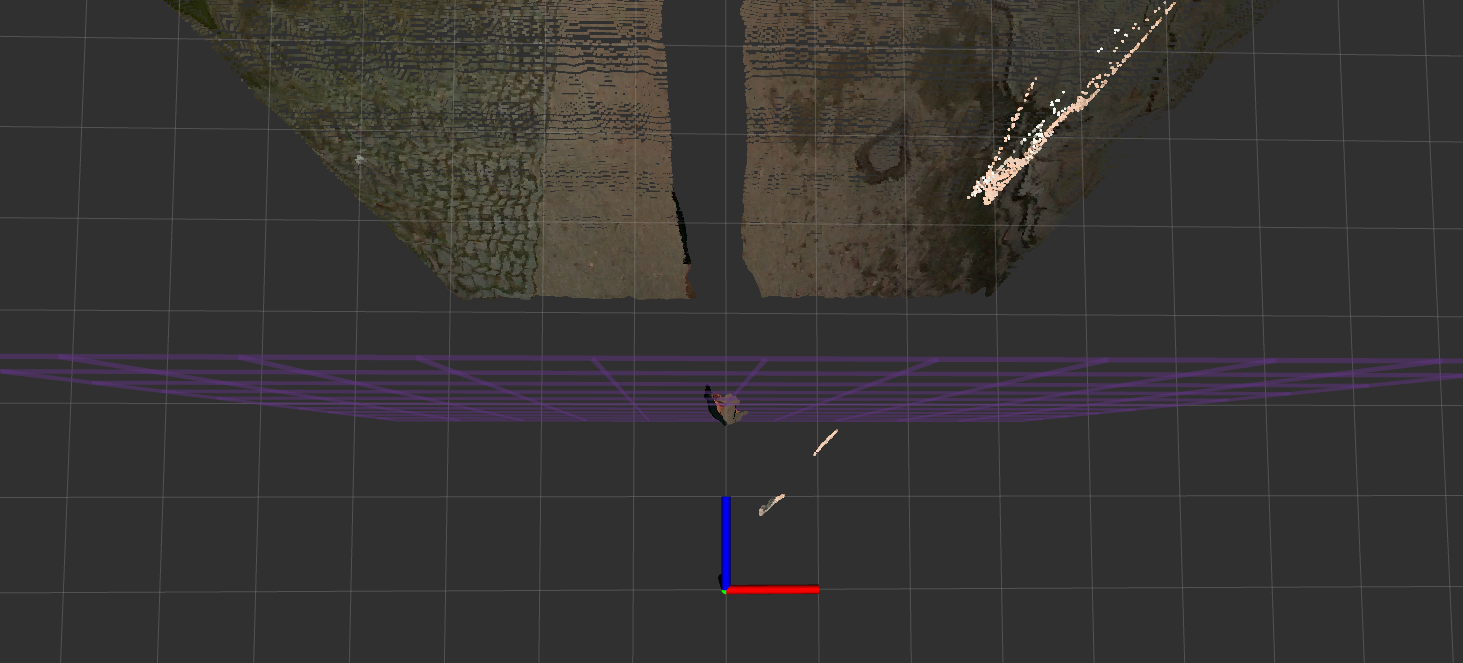
\includegraphics[width=0.7\textwidth]
  {figures/framosEval/session1/depthResults3D/2_1.png}
  \caption{3D depth visualization at 2\,m distance.}
  \label{fig:app_2m_3d}
\end{figure}

\begin{figure}[H]
  \centering
  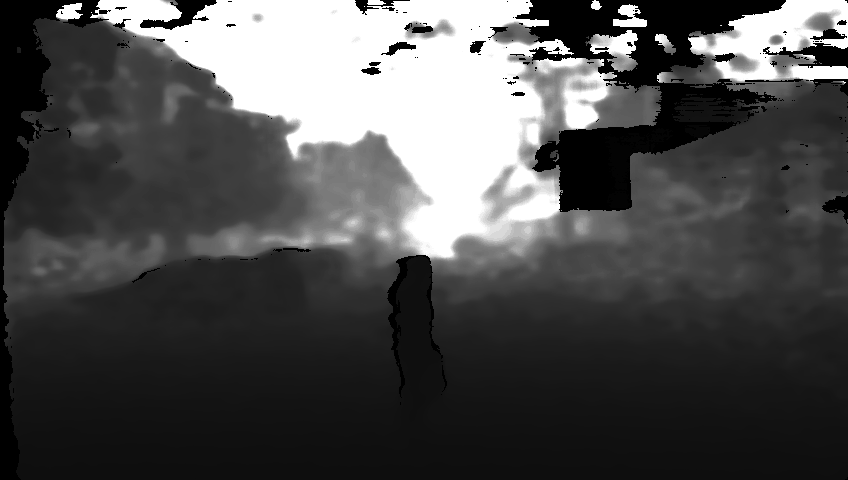
\includegraphics[width=0.7\textwidth]
  {figures/framosEval/session1/depthResults/4.png}
  \caption{Raw 2D depth image at 4\,m distance.}
  \label{fig:app_4m_2d}
\end{figure}

\begin{figure}[H]
  \centering
  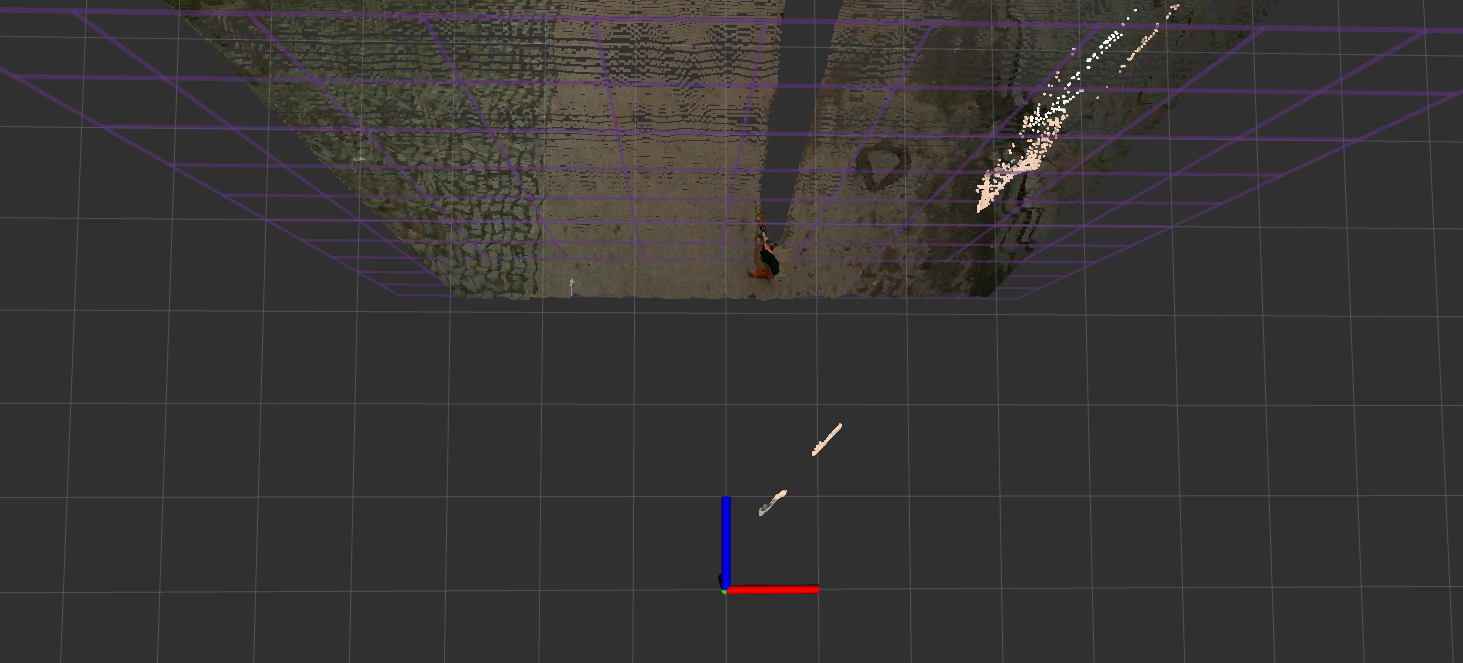
\includegraphics[width=0.7\textwidth]
  {figures/framosEval/session1/depthResults3D/4_1.png}
  \caption{3D depth visualization at 4\,m distance.}
  \label{fig:app_4m_3d}
\end{figure}

\begin{figure}[H]
  \centering
  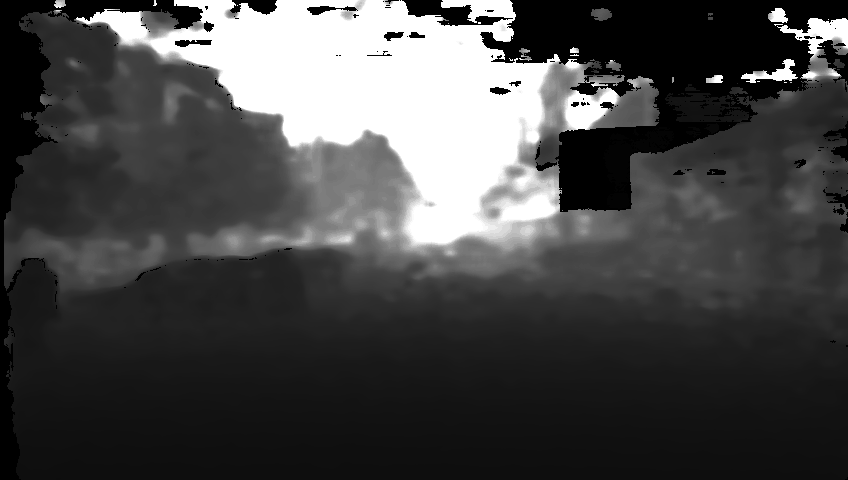
\includegraphics[width=0.7\textwidth]
  {figures/framosEval/session1/depthResults/6.png}
  \caption{Raw 2D depth image at 6\,m distance.}
  \label{fig:app_6m_2d}
\end{figure}

\begin{figure}[H]
  \centering
  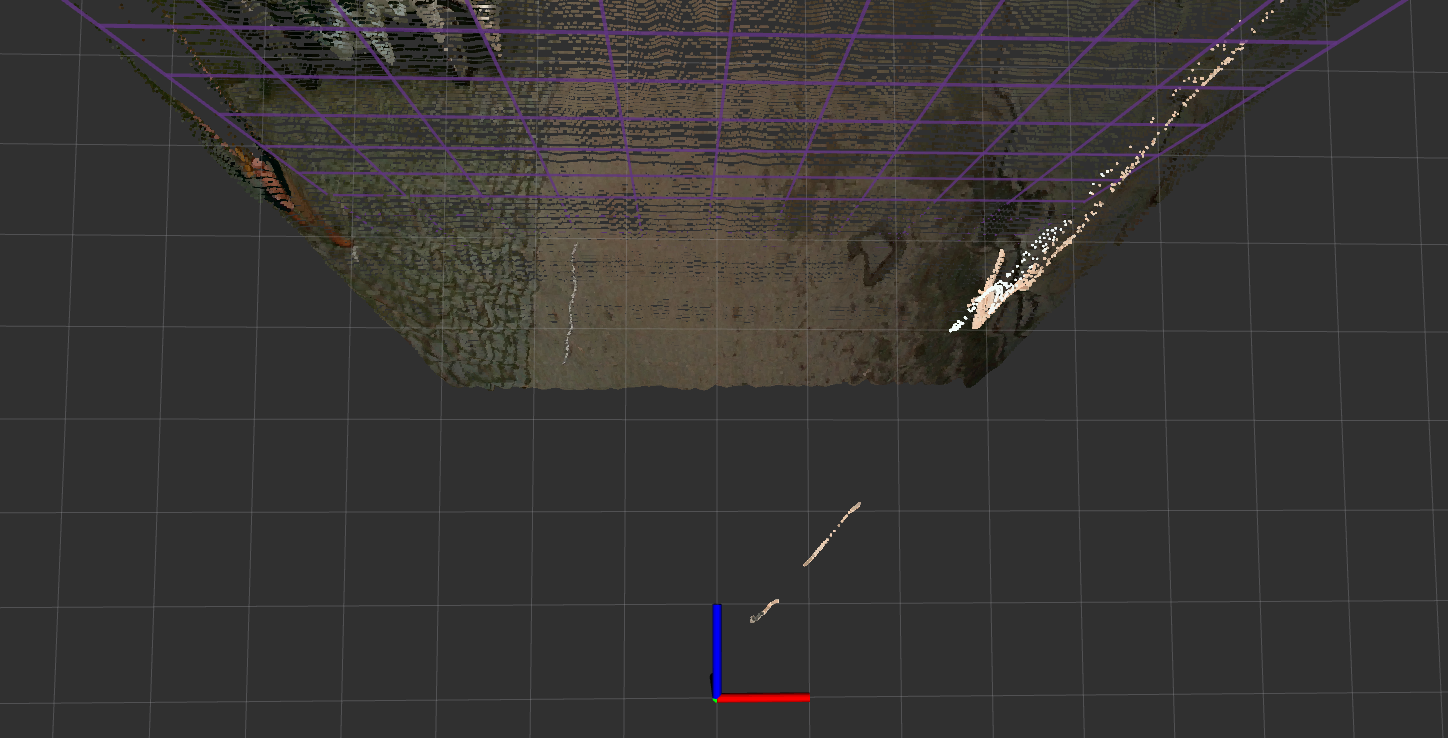
\includegraphics[width=0.7\textwidth]
  {figures/framosEval/session1/depthResults3D/6_1.png}
  \caption{3D depth visualization at 6\,m distance.}
  \label{fig:app_6m_3d}
\end{figure}

\begin{figure}[H]
  \centering
  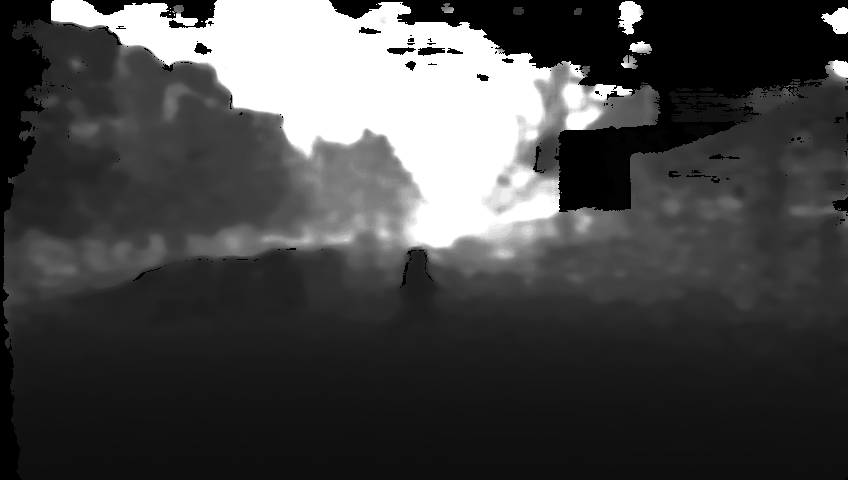
\includegraphics[width=0.7\textwidth]
  {figures/framosEval/session1/depthResults/8.png}
  \caption{Raw 2D depth image at 8\,m distance.}
  \label{fig:app_8m_2d}
\end{figure}

\begin{figure}[H]
  \centering
  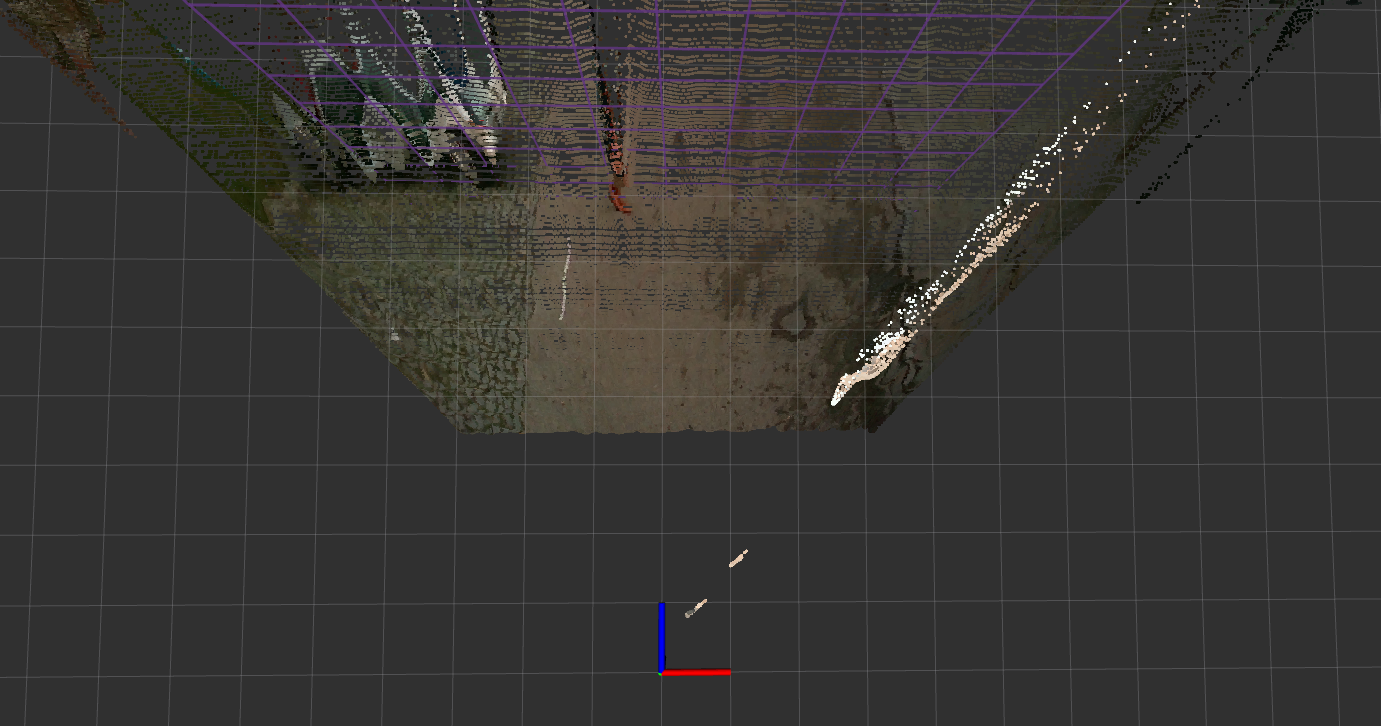
\includegraphics[width=0.7\textwidth]
  {figures/framosEval/session1/depthResults3D/8_1.png}
  \caption{3D depth visualization at 8\,m distance.}
  \label{fig:app_8m_3d}
\end{figure}

\begin{figure}[H]
  \centering
  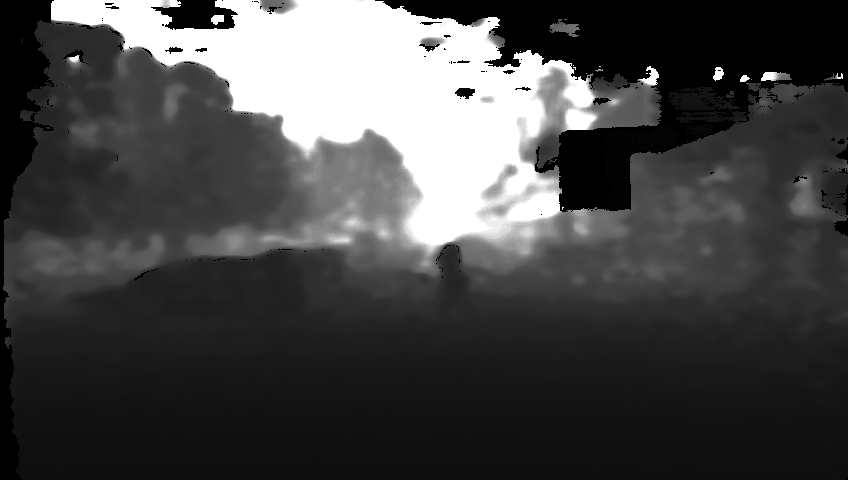
\includegraphics[width=0.7\textwidth]
  {figures/framosEval/session1/depthResults/10.png}
  \caption{Raw 2D depth image at 10\,m distance.}
  \label{fig:app_10m_2d}
\end{figure}

\begin{figure}[H]
  \centering
  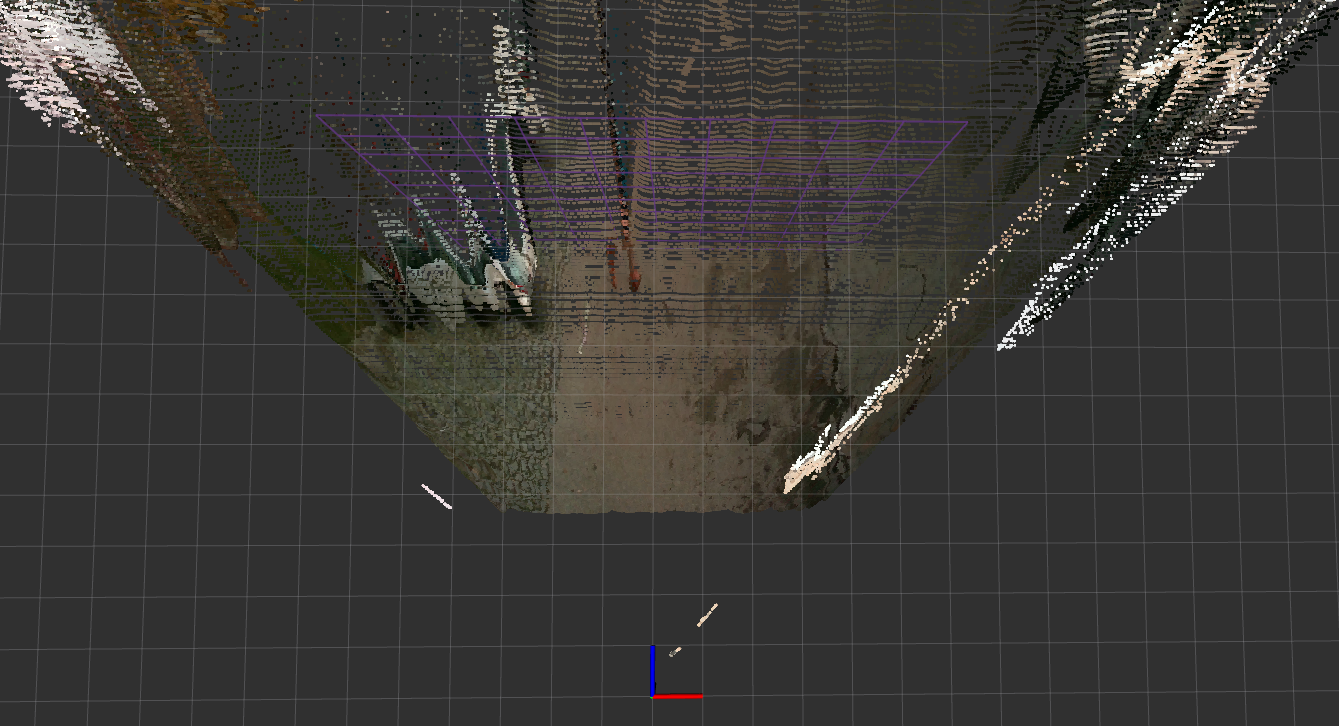
\includegraphics[width=0.7\textwidth]
  {figures/framosEval/session1/depthResults3D/10_1.png}
  \caption{3D depth visualization at 10\,m distance.}
  \label{fig:app_10m_3d}
\end{figure}

\begin{figure}[H]
  \centering
  
\includegraphics[width=0.7\textwidth]
  {figures/framosEval/session1/depthResults/12.png}
  \caption{Raw 2D depth image at 12\,m distance.}
  \label{fig:app_12m_2d}
\end{figure}

\begin{figure}[H]
  \centering
  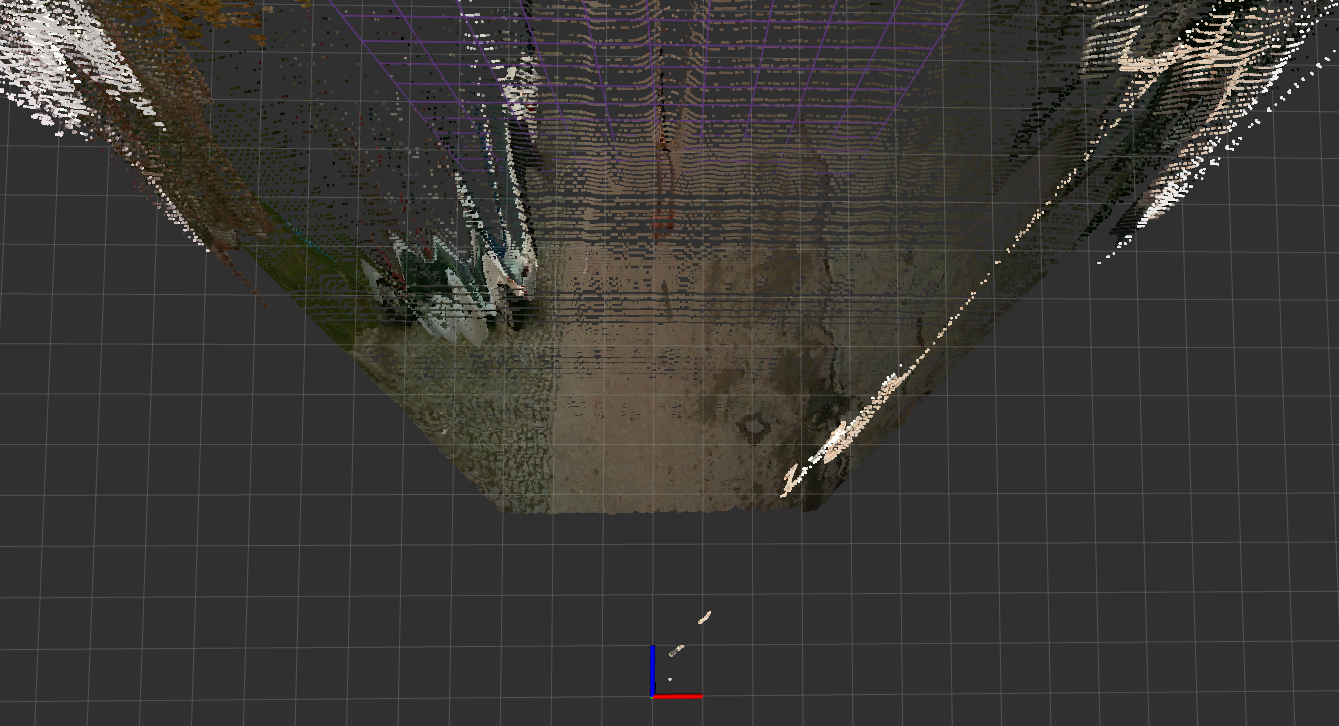
\includegraphics[width=0.7\textwidth]
  {figures/framosEval/session1/depthResults3D/12_1.png}
  \caption{3D depth visualization at 12\,m distance.}
  \label{fig:app_12m_3d}
\end{figure}
%
\end{appendices}%
%
%
\end{document}%
%
%
